\ifdefined\pdfminorversion\pdfminorversion=7\fi  % match the drawio v1.7 architecture figure (silences PDF-inclusion warning)
%==============================================================================
% CB-SAFE: full paper (IEEEtran journal / IEEE Transactions, TIFS-style). Compile:
%   pdflatex cbsafe && pdflatex cbsafe
% References are inline (thebibliography); no bibtex pass required.
% Figures are produced by experiments/plots.py into results/figs/.
%==============================================================================
\documentclass[lettersize,journal]{IEEEtran}
\IEEEoverridecommandlockouts
\usepackage{cite}
\usepackage{amsmath,amssymb}
\usepackage{booktabs}
\usepackage{rotating}
\usepackage{graphicx}
\usepackage[T1]{fontenc}
\usepackage{url}
\usepackage{array}
\usepackage{tikz}
\usetikzlibrary{arrows.meta,calc,positioning}
\usepackage[ruled,vlined]{algorithm2e}
% Float placement: let full-width (double-column) figures use dedicated float
% pages so they land near their reference instead of being flushed after the
% bibliography. stfloats matches the official IEEE TIFS template.
\usepackage{stfloats}
\renewcommand{\topfraction}{0.92}
\renewcommand{\bottomfraction}{0.85}
\renewcommand{\textfraction}{0.06}
\renewcommand{\floatpagefraction}{0.66}
\renewcommand{\dbltopfraction}{0.92}
\renewcommand{\dblfloatpagefraction}{0.66}
\setcounter{topnumber}{3}
\setcounter{bottomnumber}{2}
\setcounter{totalnumber}{4}
\setcounter{dbltopnumber}{2}
% IEEE-style blue hyperlinked citations/references (load hyperref last)
\definecolor{linkblue}{RGB}{0,0,204}
\usepackage[colorlinks=true,citecolor=linkblue,linkcolor=linkblue,urlcolor=linkblue,breaklinks=true]{hyperref}
\newtheorem{definition}{Definition}
\newtheorem{theorem}{Theorem}
\newtheorem{proposition}{Proposition}
% figure accent: one color used sparingly on top of black
\definecolor{accent}{RGB}{176,0,32}
\graphicspath{{../results/figs/}}

\begin{document}

\title{Laundering by Secure Aggregation: Temporal Group Testing for Byzantine-Robust
Federated Learning with Code-Based Post-Quantum Confidentiality}

\author{Md~Wahiduzzaman~Suva and Esm-e~Moula~Chowdhury~Abha%
\thanks{M.~W.~Suva (ID 26-94088-2) and E.~M.~C.~Abha (ID 26-94089-2) are with the
Department of Computer Science, American International University-Bangladesh,
Dhaka, Bangladesh. Corresponding author: M.~W.~Suva
(e-mail: 26-94088-2@student.aiub.edu; 26-94089-2@student.aiub.edu).}%
\thanks{Manuscript prepared September 2026. Source code, all result CSVs, and the
scripts that regenerate every table and figure are available at
\url{https://github.com/wshuv-o/cb-safe-draft}.}}

\markboth{IEEE Transactions on Information Forensics and Security,~Vol.~XX, No.~X, 2026}%
{Suva \MakeLowercase{\textit{et al.}}: CB-SAFE: Code-Based Post-Quantum Secure Aggregation for Byzantine-Robust Federated Learning}

\maketitle

\begin{abstract}
Secure aggregation reveals only the sum of federated learning (FL) updates, but its
key establishment breaks under a quantum adversary, and post-quantum FL today rests
almost entirely on lattice assumptions. We identify a \emph{laundering} effect:
aggregating securely within clusters of $c$ clients turns amplified sign-flip
poisoning into plausible-magnitude inverted cluster sums, which defeats every
coordinate-wise robust rule applied across those sums. We introduce CB-SAFE+, which
re-randomizes clustering each round and accumulates per-client suspicion from
root-anchored direction flags --- temporal group testing over private sums ---
excluding attackers the server never observes individually, using only the cluster
sums already revealed. A simulation-based privacy theorem bounds what this discloses,
against a tension we quantify: the anonymity set grows with $c$ while the probability
a cluster sum stays clean decays as $(1-f)^{c}$.
We instantiate the framework over a code-based KEM (HQC, selected by NIST in March
2025) --- to our knowledge the first Bonawitz-style masked FL aggregation on a
code-based rather than lattice KEM. The KEM is pluggable and affects only setup: on a
291\,498-parameter model with 30 clients, per-round traffic is KEM-independent and
the code-based premium is a one-time 15.2 vs.\ 3.8~KiB per masking partner at NIST
level~1, under $0.03\%$ of training traffic. Fixed clusters give $c-1$ partners, so
setup is constant in population; CB-SAFE+'s re-randomization needs secrets with all
peers, making its one-time setup $O(N)$ with per-round cost still $O(c)$.
Across CIFAR-10, FashionMNIST, EMNIST, and tabular Edge-IIoTset the laundering effect
and CB-SAFE+'s recovery replicate everywhere, and CB-SAFE+ beats every baseline under
sign-flip in a pooled paired test (Holm-corrected $p{<}0.01$). CB-SAFE+ targets
untargeted poisoning: a patch-trigger backdoor evades its direction and loss tests,
a limit we scope out rather than claim.
\end{abstract}

\begin{IEEEkeywords}
Post-quantum cryptography, federated learning, secure aggregation, HQC, code-based
cryptography, Byzantine robustness, cryptographic diversity.
\end{IEEEkeywords}

\section{Introduction}
\IEEEPARstart{F}{ederated} learning (FL) trains a shared model across many clients without
centralizing data \cite{mcmahan2017,kairouz2021}, but the transmitted model updates leak private information:
gradient-inversion \cite{zhu2019,geiping2020} and membership- or model-inversion
\cite{shokri2017,fredrikson2015} attacks reconstruct training samples from
individual updates. Secure aggregation closes this channel by ensuring the server
observes only the \emph{sum} of updates, using pairwise additive masks that cancel on
aggregation \cite{bonawitz2017,bell2020}; recent designs reduce its overhead
\cite{lightsecagg,swiftagg}, though the sum itself can still leak
\cite{elkordy2022}. The confidentiality of those masks rests on key
establishment that Shor's algorithm \cite{shor1997} breaks once a cryptographically relevant quantum
computer exists, and traffic recorded today can be decrypted then
(``harvest-now, decrypt-later'').

The standard response replaces classical key exchange with a post-quantum KEM, and
nearly all post-quantum FL does so with \emph{lattice} cryptography
\cite{pqsf2024,qinxu2025,narsimhulu2026,nguyen2025lattice,byzpqfl2026}. Lattices are
efficient and standardized (ML-KEM, FIPS~203 \cite{fips203}), but concentrating an
entire ecosystem's confidentiality on one hardness assumption is a systemic risk: a
single cryptanalytic advance would break every such deployment simultaneously. NIST
recognized exactly this risk when, in March~2025, it \emph{selected} the code-based
KEM HQC~\cite{hqc} (whose security reduces to syndrome decoding of quasi-cyclic codes
\cite{macwilliams1977}, not to lattice problems, in the tradition of code-based
cryptography since McEliece \cite{mceliece1978}) as a diversified backup to ML-KEM
\cite{nistir8545}. That diversity has not reached federated learning.

A second, orthogonal tension is that secure aggregation and Byzantine robustness pull
in opposite directions: hiding individual updates denies the server exactly the
visibility that poisoning defenses need. Recent work combines robustness with
\emph{lattice}-based post-quantum aggregation \cite{byzpqfl2026}, or achieves
cluster-based robust aggregation on \emph{quantum hardware} \cite{cqsa2026}; no prior
framework provides both under a code-based, classical post-quantum assumption.

This paper presents CB-SAFE (Code-Based Secure Aggregation for Federated
lEarning), making five contributions:
\begin{enumerate}
\item \textbf{A KEM-agnostic secure-aggregation protocol} (Definition~1) that
formalizes Bonawitz-style double masking over any IND-CCA2 KEM, with per-round mask
seeds derived from long-lived encapsulated secrets so key encapsulation is a one-time
cost. The post-quantum primitive becomes a single replaceable module.
\item \textbf{A code-based instantiation, scope-qualified:} to our knowledge, CB-SAFE
is the first FL secure-aggregation framework to obtain post-quantum confidentiality
by substituting the \emph{key-establishment KEM} in Bonawitz-style pairwise masking
with the NIST-selected code-based HQC, at matched NIST security levels. Code-based
secure aggregation as such is not new --- \cite{lpnsecagg2026} reaches it through
LPN-based homomorphic encryption --- and we claim only the KEM route, whose
distinguishing property is that the code-based premium stays a one-time setup cost.
\item \textbf{A quantified reconciliation of privacy and robustness:} secure
aggregation \emph{within} clusters of $c$ clients, robust aggregation (trimmed mean,
median, Multi-Krum) \emph{across} cluster sums, and an explicit trade-off law (the
anonymity set is $c$ while the clean-cluster probability decays as $(1-f)^c$)
validated experimentally under three attacks. We further identify and analyze a
\emph{laundering} effect: cluster averaging turns amplified sign-flip poisoning into
plausible-magnitude, direction-inverted cluster sums that defeat every
coordinate-wise robust rule (Proposition~\ref{prop:launder}).
\item \textbf{CB-SAFE+, a defense that identifies hidden attackers:} per-round
re-randomized clustering plus direction flags against a small server root dataset
accumulate per-client suspicion (temporal group testing over privacy-preserving
observations) and exclude malicious clients the server has never observed
individually. The flags are post-processing of already-revealed cluster sums, so the
defense adds \emph{no} update-content leakage beyond CB-SAFE itself (Theorem~\ref{thm:priv}).
\item \textbf{Measured cost analysis:} on a 291k-parameter model,
per-round traffic is KEM-independent and the full code-based premium is a one-time
15.2~KiB vs.\ 3.8~KiB per client (NIST level~1), i.e., $0.7\%$ of one round's
traffic and under $0.03\%$ amortized over training; HQC's $\sim$100$\times$ slower key generation at NIST level~1 contributes about 2\,s (one-time,
30 clients) versus 0.02\,s for ML-KEM.
\end{enumerate}

\section{Related Work}
\textbf{Secure aggregation.} Masking-based secure aggregation lets an
honest-but-curious server learn only the \emph{sum} of client updates. Bonawitz
\emph{et al.}\ \cite{bonawitz2017} cancel pairwise one-time masks and tolerate dropout
through secret-shared seeds; subsequent work drives down the quadratic overhead with
(poly)logarithmic-round constructions \cite{bell2020}, coded and one-shot recovery
(LightSecAgg \cite{lightsecagg}, SwiftAgg \cite{swiftagg}), and single-server
multi-round aggregation that removes the per-round setup (Flamingo \cite{flamingo}).
This entire line shares one property we must contend with: by construction the server
sees only the aggregate---which can itself still leak \cite{elkordy2022}---and never
the per-client updates that Byzantine defenses rely on. Our masked-aggregation layer
follows the same double-masking template but factors key establishment behind a
KEM-agnostic interface, so a code-based post-quantum KEM substitutes for the classical
one in a single module.

\textbf{Post-quantum FL is lattice-dominated.} PQSF reconstructs masks with lattice
multi-stage secret sharing \cite{pqsf2024}; Qin and Xu build single-round aggregation
from a lattice key-homomorphic PRF \cite{qinxu2025}; Narsimhulu \emph{et al.}
aggregate Dilithium-style lattice signatures \cite{narsimhulu2026}; and a 2026
framework combines reputation-weighted Byzantine-robust aggregation with
Kyber/lattice-based secure aggregation for IoT threat intelligence
\cite{byzpqfl2026}. Surveys confirm lattice dominance across post-quantum deployment
\cite{nguyen2025lattice}. Non-lattice exceptions are few: multivariate
cryptography with blockchain \cite{singh2025pqfog}, and CQSA, which partitions
clients into clusters aggregated via GHZ states on near-term \emph{quantum hardware}
\cite{cqsa2026}. Code-based constructions are not absent, however. Closest is
\cite{lpnsecagg2026}, which builds secure aggregation from key- and
message-additive homomorphic encryption under Learning Parity with Noise and treats
the multi-round FL setting explicitly. That work and ours reach code-based
confidentiality by different routes: it replaces the aggregation primitive with an
LPN-based homomorphic scheme, whereas we keep Bonawitz-style pairwise masking and
replace only the key-establishment KEM, which is what lets the same protocol run
unchanged over HQC or ML-KEM and makes the code-based premium a one-time setup cost
rather than a per-round one. Our claim is therefore scoped to the KEM route, not to
code-based secure aggregation in general. CB-SAFE differs from the lattice work on the confidentiality
assumption: syndrome decoding of quasi-cyclic codes, via a standard-track classical
KEM \cite{nistir8545}, with the KEM exposed behind an agnostic interface so lattice
and code-based variants differ in exactly one module.

\textbf{Byzantine robustness and poisoning.} Model- and data-poisoning attacks
\cite{fang2020,shejwalkar2021,tolpegin2020}, including stealthy \cite{baruch2019}
and backdoor \cite{bagdasaryan2020,wangtails2020} variants, and their defenses are a
large literature: robust aggregation rules such as Multi-Krum \cite{blanchard2017},
coordinate-wise trimmed mean and median \cite{yin2018}, Bulyan \cite{bulyan}, and the
geometric-median aggregator RFA \cite{rfa}; trust-bootstrapped filtering
(FLTrust \cite{fltrust}, Zeno \cite{zeno}); malicious-client detection, including
recent 2025--26 methods (FLDetector \cite{fldetector2022}, FLAegis \cite{flaegis2025},
SafeFL \cite{safefl2025}, and loss-trend monitoring \cite{flltd2026}, whose
temporal-loss signal parallels our root-loss probe); and backdoor-specific defenses
(FLAME \cite{flame2022}). These detectors inspect \emph{individual} client updates,
which secure aggregation deliberately hides. A parallel line enforces robustness or
integrity \emph{on the masked updates themselves}---zero-knowledge norm and
well-formedness proofs (RoFL \cite{rofl}), verifiable secret-shared integrity checks
(EIFFeL \cite{eiffel}), and two-server distributed-trust aggregation that withstands
malicious clients (ELSA \cite{elsa})---but these are classical (pre-quantum) and
\emph{bound or validate} updates rather than identifying the responsible clients.
Privacy-preserving robust aggregators
narrow that gap (PriRoAgg \cite{priroagg2024}, Giskard \cite{giskard2026}), but obtain
confidentiality from lattice/MPC rather than a post-quantum code-based KEM and do not
identify individual attackers. This is the privacy--robustness--post-quantum tension we
address.

\textbf{Cluster-based robust aggregation.} Reconciling Byzantine resilience
with secure aggregation is an established goal: BREA does so through
secret-shared distance computation \cite{brea2021}, CQSA through clustered
aggregation on quantum hardware \cite{cqsa2026}, and, closest to our robustness
mechanism, FedGT \cite{fedgt} identifies malicious clients by non-adaptive group
testing \cite{dorfman1943,aldridge2019} over overlapping secure-aggregation groups,
decoding a fixed parity-check assignment with a per-round BCJR decoder~\cite{bcjr} whose code is
designed for a small, fixed population ($n{\le}31$). Aggregating within groups and
inspecting group sums is thus a known structure; our contribution is not the cluster
topology itself but (i) its first classical post-quantum, code-based
instantiation and (ii) an explicit, experimentally validated statement of the
privacy--robustness trade-off it induces (Section~\ref{sec:tradeoff}), with a
temporal group-testing defense (CB-SAFE+) that matches FedGT's attacker
identification at far lower false-positive cost, and scales past FedGT's fixed
small-population design.

Across this landscape, existing
post-quantum FL is lattice-based and, with one recent exception \cite{byzpqfl2026},
not Byzantine-robust; classical robust-aggregation and detection methods are neither
post-quantum nor compatible with secure aggregation; and FedGT---the closest design---is
neither post-quantum nor scalable beyond its fixed $n{\le}31$ code. CB-SAFE+ is, to our
knowledge, the only framework that is simultaneously code-based post-quantum,
secure-aggregating, Byzantine-robust, identifies malicious clients, and scales.

\section{The CB-SAFE Framework}

\begin{figure*}[tp]
\centering

\includegraphics[width=\textwidth]{fig_architecture.pdf}
\caption{CB-SAFE, one training round end to end: one-time HQC key setup,
within-cluster masked aggregation (the server sees only the $k$ cluster sums), and
the CB-SAFE+ flag/exclude stage.}
\label{fig:arch}
\end{figure*}

\subsection{Notation}
We use lowercase bold for vectors and uppercase bold for matrices. The server
coordinates $N$ clients grouped into clusters of size $c$; a fraction $f$ is
malicious.

\subsection{System and Threat Model}
A server coordinates $N$ clients running FedAvg over non-IID data partitions.
Clients are partitioned into $k=\lceil N/c\rceil$ clusters of size $c$. The server is
honest-but-curious; a fraction $f$ of clients are malicious and submit poisoned
updates; clients may drop out mid-round. Within a cluster, mask recovery uses a
$t$-of-$c$ threshold with $t=\lfloor c/2\rfloor+1$, so privacy holds against the
server colluding with up to $t-1$ members of a cluster, and any $c-t$ members can
drop without stalling the round. Update authentication is out of the code-based
scope: HQC cannot sign and no code-based signature is standardized, so where
signatures are required we compose the lattice-based ML-DSA \cite{fips204} and state
explicitly that only the confidentiality layer is code-based.

\subsection{KEM-Agnostic Masked Aggregation}
\begin{definition}[KEM-agnostic cluster masking]\label{def:kem}
Let $\mathcal{K}=(\mathrm{KeyGen},\mathrm{Encaps},\mathrm{Decaps})$ be an IND-CCA2
KEM, $H$ a key-derivation function, and $G$ a PRG into $(\mathbb{Z}_{2^{64}})^d$.
At setup, each client $i$ publishes $pk_i$; for each cluster pair $i<j$, client $i$
computes $(ct_{ij}, ss_{ij})=\mathrm{Encaps}(pk_j)$ and $j$ recovers
$ss_{ij}=\mathrm{Decaps}(sk_j, ct_{ij})$. In round $r$, client $i$ quantizes its
update $x_i$ to $q(x_i)\in(\mathbb{Z}_{2^{64}})^d$, draws a self-mask seed $b_i^r$,
Shamir-shares it $t$-of-$c$ within its cluster, and submits
\begin{equation}\label{eq:mask}
\mathbf{y}_i = q(\mathbf{x}_i) + G(b_i^r) + \!\sum_{j>i}\! G\!\big(H(ss_{ij}, r)\big)
      - \!\sum_{j<i}\! G\!\big(H(ss_{ij}, r)\big) \!\!\!\pmod{2^{64}},
\end{equation}
where the sums run over the cluster peers of $i$. The server adds each cluster's
submissions (pairwise masks cancel), reconstructs each survivor's $b_i^r$ from $t$
shares and removes $G(b_i^r)$; for a dropped client $d$, each survivor $j$ reveals
the per-round seed $H(ss_{dj}, r)$ and the server removes the orphaned mask halves.
The server thus obtains exactly $\sum_{i \in \mathrm{alive}} q(x_i)$ per cluster.
\end{definition}

Correctness is exact: masking is modular-arithmetic exact, and the only deviation
from plain float aggregation is fixed-point quantization ($2^{-16}$ per coordinate).
Because encapsulation happens once and per-round seeds come from $H(ss_{ij}, r)$,
per-round messages contain no KEM material at all: the masked update is $8d$ bytes
regardless of the KEM, and the KEM's key and ciphertext sizes appear only in the
one-time setup. Instantiating $\mathcal{K}$ with HQC gives the code-based variant;
with ML-KEM \cite{fips203}, the lattice baseline.

\begin{algorithm}[t]
\caption{Cluster Secure Aggregation (round $r$)}
\label{alg:secagg}
\DontPrintSemicolon
\KwIn{cluster $C$ of size $c$, threshold $t$, per-pair secrets $\{ss_{ij}\}$}
\KwOut{cluster sum $\textstyle\sum_{i\in\mathrm{alive}} q(\mathbf{x}_i)$}
\ForEach{client $i \in C$}{
  $q(\mathbf{x}_i) \leftarrow$ quantize local update\;
  draw self-mask seed $b_i^r$; Shamir $t$-of-$c$ share it to peers\;
  send masked $\mathbf{y}_i$ by Eq.~\eqref{eq:mask}\;
}
$Y \leftarrow \sum_{i\in\mathrm{alive}} \mathbf{y}_i$ \tcp*{pairwise masks cancel}
\ForEach{survivor $i$}{reconstruct $b_i^r$ from $t$ shares; $Y \leftarrow Y - G(b_i^r)$\;}
\ForEach{dropout $d$}{survivors reveal $H(ss_{dj},r)$; remove orphaned mask halves from $Y$\;}
\Return $Y$\;
\end{algorithm}

\begin{theorem}[Privacy against honest-but-curious coalitions]\label{thm:priv}
Assume $\mathcal{K}$ is IND-CCA2, $H$ is a secure KDF, and $G$ is a secure PRG. Fix
a cluster $C$ of size $c$ with threshold $t=\lfloor c/2\rfloor+1$, and let the
adversary $\mathcal{A}$ comprise the honest-but-curious server and any statically
chosen $T \subset C$ with $|T| \le t-1$ (the corruption set is fixed before the
protocol runs; we do not claim adaptive-corruption security). There exists a PPT simulator that, given only the corrupted
clients' inputs and the sum $\sum_{i \in \mathrm{alive}(C)\setminus T} q(x_i)$,
produces a view computationally indistinguishable from $\mathcal{A}$'s view of a
CB-SAFE round. The CB-SAFE+ flag bits are a deterministic function of the revealed
cluster sums and server-local data, so CB-SAFE+ leaks nothing beyond CB-SAFE.
\end{theorem}

\emph{Proof sketch.} A hybrid argument. (H1) Replace each pairwise secret $ss_{ij}$
between honest clients by a uniform string: distinguishing H1 from the real game
breaks IND-CCA2 of $\mathcal{K}$. (H2) Replace the per-round seeds $H(ss_{ij},r)$
and mask streams $G(\cdot)$ by uniform: breaks the KDF/PRG. In H2 every honest
submission $y_i$ is uniform subject to the alive-honest submissions summing to the
revealed cluster sum, which the simulator can sample directly. Shamir shares held by
$\le t-1$ corrupted parties are uniform by perfect secrecy below the threshold, and
a dropped client's revealed seeds $H(ss_{dj}, r)$ are independent of other rounds'
seeds under the KDF assumption, so both recovery paths are simulatable. Distinct
rounds use distinct seeds, so views compose across rounds. \hfill$\square$

The anonymity set of an honest client is therefore its cluster's alive honest-member
count, and re-randomizing the partition each round (CB-SAFE+) does not change the
per-round argument because each round reveals sums of fresh, independently masked
updates.

\textbf{What this theorem does not cover.} Three limits deserve stating plainly,
because the per-round guarantee is weaker than it may read.

\emph{(i) Cross-round composition.} Masks are independent across rounds, but
\emph{updates} are not: a client trains on the same local data every round, so its
contributions are strongly correlated. Over $R$ rounds CB-SAFE+ places that client
with different partners each time, so the server observes $R$ different $c$-party sums
each containing an approximately repeated vector. That is the same linear-system
structure the fixed-cluster design refuses within a round, spread across rounds.
CB-SAFE+ is itself evidence that it carries signal: the defense works precisely by
inferring a per-client property (maliciousness) from cross-round group sums, and the
same channel is open to an honest-but-curious server pursuing other per-client
properties. The correct statement is therefore narrower than ``no privacy is spent'':
CB-SAFE+ reveals no update \emph{content} beyond the cluster sums CB-SAFE already
exposes, but re-randomizing those sums over time is deliberately informative about
individual clients. Quantifying what else is recoverable that way is open.

\emph{(ii) The server chooses the partition.} Our anonymity-set argument assumes the
partition is drawn honestly. A curious server colluding with one client can instead
place that colluder with a target every round, reducing the target's effective
anonymity set to the remaining $c-2$ honest members --- one, at $c{=}3$. Making the
partition verifiably random (a shared randomness beacon, or a VRF over a public seed)
closes this and is compatible with the protocol as specified; we assume it rather
than implement it.

\emph{(iii) The anonymity set is small.} At $c{=}3$ the server sees sums of three
updates, or two with one colluder. Gradient-inversion attacks \cite{zhu2019} are known
to succeed on aggregates of this size, so ``sums rather than updates'' should not be
read as strong protection at small $c$. We do not run an inversion attack on the
revealed cluster sums; doing so would turn the privacy side of the
privacy--robustness dial into a measured quantity rather than an asserted one, and is
the experiment we would add next.

\subsection{Robust Aggregation Across Cluster Sums}\label{sec:tradeoff}
The server sees $k$ cluster sums $S_1,\dots,S_k$ (means after dividing by alive
counts) and no individual update. CB-SAFE applies a robust rule across the cluster
means: coordinate-wise trimmed mean (trim $\beta$ per side) or median \cite{yin2018},
Multi-Krum \cite{blanchard2017}, Bulyan \cite{bulyan}, or the geometric median
(RFA) \cite{rfa}. This resolves the hide-versus-inspect tension structurally (privacy
is enforced below the cluster boundary, robustness operates above it) at a
quantifiable price. A cluster mean is contaminated if it contains at least one
malicious member, so with malicious fraction $f$ and random cluster assignment,
\begin{equation}\label{eq:contam}
\Pr[\text{cluster clean}] = (1-f)^{c},
\end{equation}
and the expected number of clean cluster means is $k(1-f)^c$. Larger $c$ improves
privacy (bigger anonymity set) but shrinks the clean fraction the robust rule can
rely on; a trimmed mean discarding $\beta$ per side tolerates at most
$\lfloor \beta k \rfloor$ contaminated clusters. $c$ is therefore a tunable
privacy--robustness dial, and Section~\ref{sec:eval} traces its consequences
empirically. Setting $c{=}1$ recovers classical (privacy-free) robust aggregation;
setting $c{=}N$ recovers full secure aggregation with no robustness.

The contamination probability, however, understates the problem: cluster averaging
also \emph{disguises} what it contaminates.

\begin{proposition}[Laundering by cluster averaging]\label{prop:launder}
Let each honest update be $h$ (up to noise) and let $m$ members of a cluster of size
$c$ submit the scaled sign-flip $-\gamma h$. The cluster mean is
$\mu = \frac{c - m(1+\gamma)}{c}\, h$. Its magnitude equals an honest cluster's
($|\mu| = |h|$) exactly when $\gamma = 2c/m - 1$, while its direction is inverted.
At the common attack setting $\gamma{=}5$ with $c{=}3$, $m{=}1$ this holds with
equality: the poisoned cluster sum is indistinguishable from honest by any
magnitude- or order-statistic test, and a near-symmetric $\pm h$ population drives
coordinate-wise trimmed mean and median toward $0$, stalling learning entirely.
\end{proposition}

This laundering effect explains the empirical collapse of every coordinate-wise
rule in Section~\ref{sec:eval} and motivates direction-based detection: what
cluster averaging cannot hide is the \emph{sign} of the update. The proposition
idealizes honest updates as a common $h$; under non-IID heterogeneity real honest
updates vary, so it predicts the boundary $\gamma^{*}$ in the mean rather than
exactly per cluster. We therefore read the four-dataset collapse as strong
empirical validation \emph{near} that boundary, not as a guarantee of collapse for
arbitrary honest-update distributions.

\begin{figure}[tbp]
\centering
\begin{tikzpicture}[>=Stealth,line width=0.5pt]
  \def\R{1.7}
  % axes (thin, gray)
  \draw[gray!45,->] (-3.0,0) -- (3.0,0);
  \draw[gray!45,->] (0,-2.2) -- (0,2.2);
  % circle of radius |h|
  \draw[dashed,gray!65] (0,0) circle (\R);
  \node[gray!55,font=\scriptsize] at (48:\R) {$|\mathbf{h}|$};
  % honest updates (black): the c-m clean members near +h
  \draw[->,black] (0,0) -- (34:\R) node[right,font=\scriptsize] {$\mathbf{h}$};
  \draw[->,black!60] (0,0) -- (21:\R);
  % single amplified sign-flip -gamma h (accent), truncated with a scale break
  \draw[->,accent] (0,0) -- (214:2.45);
  \draw[accent] (214:1.05)++(-0.06,0.09) -- ++(0.12,-0.18);
  \draw[accent] (214:1.22)++(-0.06,0.09) -- ++(0.12,-0.18);
  \node[accent,font=\scriptsize] at (214:2.75) {$-\gamma\mathbf{h}$};
  % resulting cluster mean mu = -h (accent): same magnitude, inverted direction
  \draw[->,accent] (0,0) -- (214:\R) node[below,font=\scriptsize] {$\boldsymbol{\mu}$};
\end{tikzpicture}
\caption{Laundering geometry (schematic). Averaging $c{-}m$ honest updates
$\mathbf{h}$ with $m$ sign-flips $-\gamma\mathbf{h}$ gives
$\boldsymbol{\mu}=\tfrac{c-m(1+\gamma)}{c}\,\mathbf{h}$; at $\gamma^{\!*}{=}2c/m-1$ it
matches $|\mathbf{h}|$ with opposite sign (Proposition~\ref{prop:launder}).}
\label{fig:launder-geom}
\end{figure}

\subsection{CB-SAFE+: Temporal Group Testing over Cluster Sums}\label{sec:defense}
CB-SAFE+ turns the laundering signature into an identification mechanism, using
three ingredients. (i)~\emph{Re-randomized clustering, one partition per round}: the
server draws a \emph{single} fresh partition of the active clients into size-$c$
clusters each round (pairwise secrets with all peers are established once at setup, so
re-clustering adds no per-round KEM cost). Using \emph{one} partition per round is a
privacy requirement, not merely a convenience: it reveals exactly one size-$c$ cluster
sum per client (rank $c$), whereas placing a client in $o$ groups
\emph{simultaneously} would reveal $o$ overlapping sums of the same update and make the
round's linear system solvable, defeating Theorem~\ref{thm:priv}. The overlap that
group testing needs is instead obtained \emph{across} rounds (ingredient~iii).
(ii)~\emph{Loss-probe flags}: the server maintains a small root dataset
($|\mathcal{D}_0|{=}200$ samples held out from all clients, the standard
trust-bootstrapping assumption \cite{fltrust,zeno}), applies each cluster mean
$\mathbf{S}_\ell$ to the current model $\theta^r$, and records the change in root loss
$\Delta_\ell^{\,r}=L(\theta^r+\mathbf{S}_\ell;\,\mathcal{D}_0)-L(\theta^r;\,\mathcal{D}_0)$.
An absolute $\Delta_\ell>0$ test over-flags, because an honest non-IID cluster mean can
itself raise the loss slightly on a small balanced root set; we therefore flag
\emph{relative to the cleanest cluster of the round},
\begin{equation}\label{eq:flag}
g_\ell^{\,r} = \mathbb{1}\!\left[\, \Delta_\ell^{\,r} \;>\; \min_{k}\Delta_k^{\,r} + \delta \,\right],
\end{equation}
with a small margin $\delta$: a $\gamma$-amplified ascent direction spikes
$\Delta_\ell$ far above the cleanest cluster no matter whose data dominates the sum.
Flags are computed from already-revealed cluster sums
and server-local data, so they reveal no update content beyond those sums
(Theorem~\ref{thm:priv}). The probe is
the product of two measured failures. Anchor-free direction flags are
sign-ambiguous: the poisoned cluster sums form their own coherent cloud at $-h$, and
a Krum-based reference locks onto that cloud in a large fraction of rounds.
Anchored \emph{cosine} flags break the symmetry but lose specificity under non-IID
data: an $m{=}1$ poisoned cluster mean is dominated by $-\gamma$ times one client's
idiosyncratic direction, nearly orthogonal to the balanced anchor, so its sign test
approaches a coin flip (at $f{=}0.2$ we measured cosine flags hitting clean clusters
as often as dirty ones, and suspicion never separated). The loss probe is immune to
this decorrelation because a $\gamma$-amplified ascent direction raises root loss
regardless of whose data dominates the cluster sum. (iii)~\emph{Temporal group
testing and adaptive exclusion}: across $o$ consecutive rounds a client is
re-clustered into $o$ different groups, the across-round analog of $o$ overlapping
tests. A client accrues a suspicion mark in round $r$ only if its cluster was flagged
in \emph{every} one of the last $o$ rounds (a windowed combinatorial orthogonal
matching pursuit (COMP) decode~\cite{comp}); writing
$G_i^{\,r}=\prod_{\rho=r-o+1}^{r} g_{\ell(i,\rho)}^{\,\rho}$ for that windowed
conjunction ($o{=}1$ recovers plain per-round accumulation), after $r$ rounds client
$i$ has accumulated
\begin{equation}\label{eq:susp}
s_i^{\,r} = \sum_{\rho\le r} G_i^{\,\rho}.
\end{equation}
A malicious client accumulates suspicion far faster than an honest one---its flagged
fraction plateaus near $0.73$ in our runs---while an honest client is flagged only when
randomly co-clustered with an attacker, with per-round probability
\begin{equation}\label{eq:ph}
p_h = 1-(1-f)^{\,c-1} < 1 ,
\end{equation}
and only $p_h^{\,o}$ across a full window, so overlap further suppresses honest false
positives. After a warmup of $W$ rounds the server excludes clients by an
\emph{adaptive gap} rather than a fixed cut: it sorts the flagged fractions
$s_i^{\,r}/r$, takes the largest gap between consecutive values, and excludes the high
side when that gap exceeds a minimum separation, its midpoint $\sigma^{*}$ sits above a
floor, and the excluded set is a minority,
\begin{equation}\label{eq:excl}
\text{exclude } i \iff r>W \ \text{and}\ s_i^{\,r}/r > \sigma^{*} .
\end{equation}
A fixed threshold $\tau$ is deliberately avoided: a $\gamma$-amplified attacker can
plateau its flagged fraction just below any preset $\tau$ (we observed $\sim$0.73
against $\tau{=}0.85$) and evade the cut, whereas the gap rule keys on the
\emph{separation} between the honest and malicious populations, which is present
whenever an attack is. By Hoeffding's inequality those populations concentrate near
$p_h^{\,o}$ and $1$ and separate exponentially, so a few rounds open a gap wide enough
to cut, as the measured suspicion trajectories confirm (Fig.~\ref{fig:suspicion}).
The server thereby identifies individual attackers it has never observed
individually: group testing \cite{dorfman1943,aldridge2019} whose pools are the
privacy-preserving cluster sums and whose tests repeat, and overlap, over training
rounds. At large populations ($N>N_0{=}50$) per-client data shrinks, so absolute loss
deltas compress and the suspicion histogram densifies; the flag and the exclusion then
switch to scale-invariant robust rules (upper median-plus-MAD outliers), which is what
keeps CB-SAFE+ effective at $N{=}500$ (Section~\ref{sec:eval}).

\begin{algorithm}[t]
\caption{CB-SAFE+: Temporal Group Testing over Cluster Sums}
\label{alg:cbsafeplus}
\DontPrintSemicolon
\KwIn{clients $[N]$, root $\mathcal{D}_0$, cluster size $c$, overlap $o$, warmup $W$, flag margin $\delta$, rounds $R$}
\KwOut{global model $\theta$, excluded set $\mathcal{E}$}
$s_i \leftarrow 0$, window $h_i \leftarrow (\,)\ \forall i$;\quad $\mathcal{E}\leftarrow\varnothing$\;
\For{$r \leftarrow 1$ \KwTo $R$}{
  redraw \emph{one} random partition of $[N]\setminus\mathcal{E}$ into clusters of size $c$\;
  \lForEach{cluster $\ell$}{$\mathbf{S}_\ell \leftarrow \textsc{ClusterSecureAgg}(\ell,r)/|\mathrm{alive}(\ell)|$;\ \ $\Delta_\ell \leftarrow L(\theta{+}\mathbf{S}_\ell;\mathcal{D}_0){-}L(\theta;\mathcal{D}_0)$}
  \lForEach{cluster $\ell$}{$g_\ell \leftarrow \mathbb{1}[\Delta_\ell > \min_k\Delta_k + \delta]$}\tcp*{Eq.~\eqref{eq:flag}}
  \ForEach{active client $i$, in its cluster $\ell$}{
    append $g_\ell$ to $h_i$ and keep its last $o$ entries\;
    \lIf{$|h_i|{=}o$ \textup{and} $\min h_i{=}1$}{$s_i \leftarrow s_i{+}1$}\tcp*{windowed COMP}
  }
  \lIf{$r > W$}{$\mathcal{E}\leftarrow\mathcal{E}\cup\textsc{GapExclude}\big(\{s_i/r\}\big)$}\tcp*{adaptive gap, Eq.~\eqref{eq:excl}}
  $\theta \leftarrow \theta + \textsc{RobustAgg}\big(\{\mathbf{S}_\ell : g_\ell{=}0\}\big)$\;
}
\Return $\theta,\ \mathcal{E}$\;
\end{algorithm}

\section{Implementation}
CB-SAFE is implemented in Python on liboqs~0.15.0 (via \texttt{liboqs-python}) and
PyTorch, with the KEM selected by a one-line configuration change among HQC-128/192/256
and ML-KEM-512/768/1024 (Kyber round-3 parameter sets are retained for comparison
with older literature). Masks are ChaCha20~\cite{chacha20} keystreams; per-round seeds use
HKDF-SHA256~\cite{hkdf}; self-mask seeds are shared with Shamir's scheme~\cite{shamir1979} over
$\mathrm{GF}(2^{127}-1)$. \emph{HQC provenance:} liboqs~0.15.0 ships the PQClean
constant-time implementation of the Round-4 HQC specification~\cite{hqc} (2023-04-30), the
version NIST evaluated and selected \cite{nistir8545}; the finalized standard's
parameters may differ slightly once published (a draft is expected as FIPS~207).
Federated training is simulated in-process; every protocol byte count and crypto
timing reported below is measured from real objects on the wire path of the
protocol (public keys, ciphertexts, shares, masked vectors), not modeled.
One training round of 30 clients takes $\approx$21\,s on the RTX 2060; the full
software and hardware configuration is given once in Section~\ref{sec:eval}.

\section{Evaluation}\label{sec:eval}
\subsection{Setup}
\textbf{Task and data.} Primary task: CIFAR-10 partitioned across $N{=}30$ clients
by a Dirichlet($\alpha{=}0.5$) label-skew split; a CNN with $d{=}291\,498$
parameters; one local epoch per round (SGD, lr $0.01$, momentum $0.9$, batch $64$);
$k{=}10$ clusters of $c{=}3$ unless stated. The split is sharply non-IID: clients
hold $631$ to $3298$ samples with strongly skewed label distributions, the
heterogeneity under which all robustness results are reported.

Generalization (Section~\ref{sec:general})
adds FashionMNIST (same CNN), EMNIST-balanced (47 classes), and Edge-IIoTset (a 15-class tabular IoT
intrusion-detection set with a multilayer perceptron), each Dirichlet-partitioned
identically. \textbf{Configurations.} Plain FedAvg (no
cryptography); CB-SAFE/lattice (ML-KEM); CB-SAFE/code-based (HQC), at matched NIST
levels. \textbf{Attacks.} Label flipping ($y \to 9-y$), sign flipping
($-5\Delta$), and a backdoor \cite{bagdasaryan2020} (3$\times$3 trigger patch,
target class~0, 50\% local poison rate) at malicious fractions $f \in \{0.1, 0.2, 0.3\}$, against aggregation
rules mean, trimmed mean, median, Multi-Krum, and the CB-SAFE+ reputation defense
(Section~\ref{sec:defense}; server root set of 200 samples held out from all
clients). \textbf{Metrics.} Test accuracy;
backdoor attack success rate (ASR: fraction of triggered non-target test samples
classified as the target); communication bytes per client (setup vs.\ per-round);
crypto wall-time; dropout-recovery cost.

\textbf{Datasets and reproducibility.} The four benchmarks are CIFAR-10~\cite{krizhevsky2009} ($50{,}000$/$10{,}000$, $10$ classes), FashionMNIST~\cite{fashionmnist} ($60{,}000$/$10{,}000$, $10$ classes), EMNIST-balanced~\cite{emnist} ($112{,}800$/$18{,}800$, $47$ classes), and Edge-IIoTset~\cite{edgeiiot} (tabular IoT/IIoT intrusion detection, the \texttt{DNN-EdgeIIoT-dataset.csv} release of $2{,}219{,}201$ flows over $15$ classes, class-stratified to at most $120{,}000$ rows), each Dirichlet($\alpha{=}0.5$)~\cite{hsu2019} partitioned across $N{=}30$ clients. Unless stated: overlap degree $o\in\{1,4\}$, Shamir threshold $t{=}\lfloor c/2\rfloor{+}1{=}2$, server root $|\mathcal{D}_0|{=}200$ held out from all clients, and adaptive-gap exclusion (flag margin $\delta{=}0.25$, minimum suspicion gap $0.15$, floor $0.25$) after a warmup of $W{=}5$ rounds; for $N{>}50$ the flag and exclusion switch to robust median-plus-MAD thresholds ($1.0$ and $2.5$ MAD). KEMs span HQC-128/192/256 and ML-KEM-512/768/1024 at matched NIST levels; masks are ChaCha20 keystreams with HKDF-SHA256 per-round seeds. Runs use Python~3.12, PyTorch~2.5.0 (CUDA~12.4), and liboqs-python~0.15.0 on NVIDIA RTX~2060 (6\,GB) and RTX~5080 (16\,GB) GPUs; all results are averaged over three seeds, with significance by paired $t$-tests (Holm-corrected).

\subsection{Overhead: the Code-Based Premium Is a One-Time Cost}
Table~\ref{tab:overhead} reports measured per-client traffic and crypto time.
Per-round traffic is identical across all six KEMs (2\,277~KiB per client,
dominated by the $8d$-byte masked update plus 102~B of Shamir material) because
Definition~\ref{def:kem} keeps KEM objects out of the per-round path entirely. The
KEM appears only in setup: at NIST level~1, HQC costs 15.2~KiB per client against
ML-KEM's 3.8~KiB ($4.0\times$; $6.4\times$ at level~5), and 2.0\,s of one-time
compute for all 30 clients against 0.02\,s. Amortized over 40 training rounds
($\sim$89\,MiB of per-client update traffic), the code-based premium is below
$0.03\%$ of total communication (Table~\ref{tab:overhead}). A round with 10\% dropouts
adds only seed-reveal messages (32~B per survivor--dropout pair) and kept server
unmasking below 0.28\,s in all configurations.

\textbf{Dropout tolerance is a utility cost of small $c$.} With $c{=}3$ and
$t{=}\lfloor c/2 \rfloor{+}1{=}2$, a cluster survives one dropout but not two: at two
losses the threshold cannot be met and the whole cluster is discarded, taking its
surviving honest update with it. Under an i.i.d.\ dropout rate $p$ the expected
fraction of clusters lost is $\Pr[\text{2 or 3 drop}] = 3p^2(1-p)+p^3$, so $2.8\%$ of
clusters at $p{=}0.10$, $10.4\%$ at $p{=}0.20$ and $21.6\%$ at $p{=}0.30$; our
$10\%$-dropout runs discarded one of ten clusters, consistent with that. Larger $c$
both widens the anonymity set and raises the dropout budget, while lowering the
probability a cluster sum stays clean --- so dropout tolerance belongs on the same
privacy--robustness dial as $(1-f)^c$, not beside it. The practicality question that
motivated this work has a quantitative answer: \emph{cryptographic diversity in FL
secure aggregation is essentially free at the protocol level once key establishment
is amortized}: the trade-off is a one-time setup constant, not a per-round tax.

\begin{table}[t]
\caption{Measured per-client overhead ($N{=}30$, $c{=}3$, $d{=}291\,498$).
Setup is one-time; per-round traffic is KEM-independent.}
\label{tab:overhead}
\centering
\footnotesize
\setlength{\tabcolsep}{3.5pt}
\begin{tabular}{@{}lrrrr@{}}
\toprule
KEM & Setup (KiB) & Setup wall (s) & Round (KiB) & Mask (ms) \\
\midrule
ML-KEM-512  & 3.8  & 0.02 & 2\,277 & 25 \\
HQC-128     & 15.2 & 2.0  & 2\,277 & 26 \\
ML-KEM-768  & 5.6  & 0.02 & 2\,277 & 27 \\
HQC-192     & 30.8 & 5.7  & 2\,277 & 25 \\
ML-KEM-1024 & 7.7  & 0.02 & 2\,277 & 25 \\
HQC-256     & 49.4 & 10.6 & 2\,277 & 26 \\
\bottomrule
\end{tabular}
\end{table}

\subsection{Scalability in the Client Population}
Secure-aggregation cost is set by how many pairwise partners each client must
maintain. All-pairs masking~\cite{bonawitz2017} gives every client $N-1$ partners,
so per-client setup traffic and per-round mask derivation grow as $O(N)$. CB-SAFE
masks only \emph{within} clusters of size $c$, capping partners at $c-1$.

\textbf{The two variants have different setup costs, and we state them separately.}
With \emph{fixed} clusters, a client ever masks with the same $c-1$ partners, so
both quantities are \emph{constant in $N$}: extrapolating the measured HQC-128 and
ML-KEM-512 primitives (Table~\ref{tab:overhead}) by partner count, a client's
one-time setup is $15.2$~KiB (HQC) or $3.8$~KiB (ML-KEM) at any population, versus
$7.4$~MiB for all-pairs masking at $N{=}1000$ --- a $500\times$ reduction that
widens linearly with $N$.

CB-SAFE+ does not inherit that saving. Re-randomizing the partition every round
means any peer may become a cluster mate, so a client must hold a pairwise secret
with all $N-1$ peers. That establishment is one-time rather than per-round, but it
is $O(N)$: the same $7.4$~MiB at $N{=}1000$, and $3.7$~MiB at the $N{=}500$ of
Table~\ref{tab:scale-n500}. What re-randomization buys is that this cost is paid
once and the \emph{per-round} traffic stays $O(c)$ --- mask derivation over $c-1$
partners --- so the saving is in recurring bandwidth, not in setup. Since every
robustness result in Section~\ref{sec:eval} comes from CB-SAFE+, the
constant-in-$N$ setup figure should be read as applying to the fixed-cluster
configuration only. Removing this gap --- per-round encapsulation with only the new
mates, which reintroduces per-round KEM traffic, or a hash-based key tree that
derives cluster keys without all-pairs establishment --- is the obvious next step
and we do not claim it here.

Because the privacy law $\Pr[S_j\ \mathrm{clean}]{=}(1-f)^c$ and the laundering
boundary (Prop.~\ref{prop:launder}) are stated \emph{per cluster}, they are
independent of $N$. CB-SAFE therefore targets the cross-device regime where
recurring all-pairs mask derivation is infeasible.

\textbf{Robustness holds as the population scales.} Cost is only half the
scaling question; the other is whether robustness survives a $16\times$ larger
client population. We ran every rule that admits a configuration at $N{=}500$ under
sign-flip ($f{=}0.2$) for 50 rounds (Table~\ref{tab:scale-n500},
Fig.~\ref{fig:convergence-n500}). FedGT is necessarily absent here: its
parity-check matrices and prevalence-estimation tables are hardcoded for
$n{\le}31$~\cite{fedgt}, so it has no configuration at this population and cannot be
run without hand-designing new ones---a concrete scalability ceiling in the method,
not a tuning choice. At this scale each client holds only $\sim$100 samples and
attacker exclusion consumes the first $\sim$15--20 rounds, so a short 30-round
budget truncates every method mid-recovery; extending to 50 rounds lets recovery
complete and collapses the between-seed spread (from $\pm$10 to $\pm$2,
Fig.~\ref{fig:convergence-n500}). At the converged horizon CB-SAFE+ reaches
$65.7\%$ (last-five-round mean over three seeds), the coordinate-wise rules remain
laundered near chance, and FLTrust's trust weighting, which recovers fastest early,
plateaus $\sim$4 points lower ($61.3\%$) because soft down-weighting never fully
removes the laundered mass. CB-SAFE+ reaches that accuracy while excluding only
$11$ honest clients of 400 (2.75\%). Among the methods that admit a configuration at this
scale, CB-SAFE+ is the only one that pairs top-tier robustness with near-zero
honest exclusion and post-quantum security.

\begin{table}[t]
\caption{Scaling to $N{=}500$ clients (FashionMNIST, sign-flip $f{=}0.2$, 50 rounds,
Dirichlet $\alpha{=}0.5$). Test accuracy is the mean of the final five rounds over
seeds $\{0,2,3\}$ ($\pm$1 SD); honest FP is the number of honest clients (of 400)
wrongly excluded. FedGT has no configuration at this scale---its parity-check design
is hardcoded for $n{\le}31$~\cite{fedgt}, a concrete scalability ceiling. Only CB-SAFE+
holds near-clean accuracy while coordinate-wise rules collapse, without discarding
honest clients and with post-quantum security.}
\label{tab:scale-n500}
\centering
\footnotesize
\setlength{\tabcolsep}{5pt}
\begin{tabular}{@{}lccc@{}}
\toprule
Rule & Acc.\ (\%) & Honest FP\,$\downarrow$ & PQC\\
\midrule
\textbf{CB-SAFE+ (ours)} & \textbf{65.7}\,$\pm$\,2.3 & 11 & \checkmark \\
FedGT~\cite{fedgt} & $-$ (no config, $n{\le}31$) & -- & -- \\
FLTrust~\cite{fltrust} & 61.3\,$\pm$\,2.4 & -- & -- \\
Median & 25.1\,$\pm$\,7.5 & -- & -- \\
Geo-median/RFA~\cite{rfa} & 28.9\,$\pm$\,9.9 & -- & -- \\
Multi-Krum & 10.0\,$\pm$\,0.1 & -- & -- \\
Bulyan~\cite{bulyan} & 10.8\,$\pm$\,1.3 & -- & -- \\
Trimmed mean & 9.5\,$\pm$\,0.9 & -- & -- \\
Mean & 10.0\,$\pm$\,0.0 & -- & -- \\
\bottomrule
\end{tabular}
\end{table}


\begin{figure}[t]
\centering
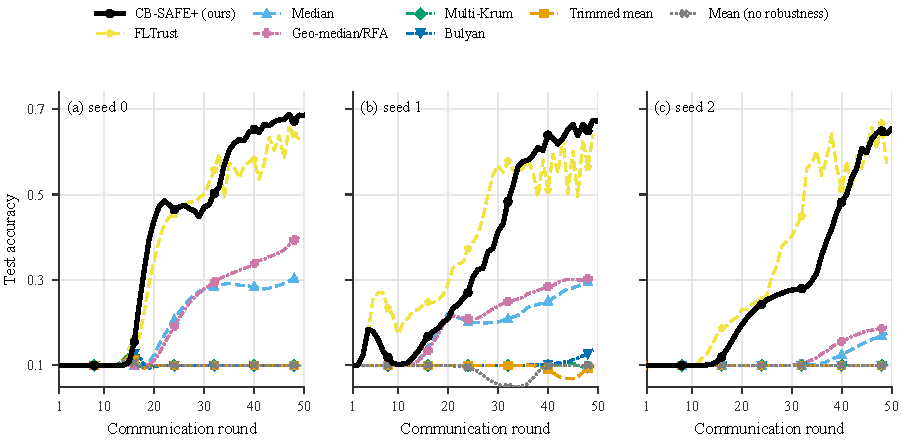
\includegraphics[width=\columnwidth]{fig_convergence_allmethods_n500.pdf}
\caption{Test accuracy vs round at $N{=}500$ (FashionMNIST, sign-flip $f{=}0.2$), one
panel per seed; eight rules (FedGT excluded, see text).}
\label{fig:convergence-n500}
\end{figure}

\subsection{Utility and Cryptographic Equivalence}
Plain FedAvg reaches 59.0\% test accuracy (mean of the final five of 40 rounds;
59.6\% at round 40) on the non-IID split. In every round,
the same client updates were pushed through the full cryptographic pipeline twice
(once under HQC-128, once under ML-KEM-768), and every per-cluster secure sum was
compared coordinate-wise against the plain sum. The maximum deviation across all 40
rounds and both KEMs was $2.28\times10^{-5}$, which \emph{equals} the worst-case
fixed-point rounding bound for a 3-element sum ($3\cdot 2^{-17}=2.29\times10^{-5}$):
the masking arithmetic itself is exact, so CB-SAFE's accuracy curve is identical to
plain FedAvg by construction, not approximately. Both dropout modes were exercised:
in round 10, two of three dropped clients landed in the same cluster, driving it
below its $t{=}2$ threshold: the protocol excluded that cluster and recovered the
remaining nine exactly; in round 20, three dropouts in three distinct clusters were
all recovered by seed-reveal plus Shamir reconstruction. Measured in-run, setup cost
2.0\,s (HQC-128) vs.\ 0.02\,s (ML-KEM-512, matched NIST level~1) for all 30 clients, and steady-state
rounds took $\sim$30\,ms of client-side masking and $\sim$0.29\,s of server-side
unmasking, negligible against the $\sim$21\,s of local training per round.

\subsection{Baseline Configuration and Where Each Rule Is Valid}\label{sec:baselines-config}
Robust rules are applied across the $k{=}\lceil N/c \rceil$ revealed cluster sums, not
across individual clients, so their own preconditions must be restated in terms of
\emph{contaminated cluster sums} rather than malicious clients. With $N{=}30$, $c{=}3$
we have $k{=}10$ inputs, and the expected number of contaminated sums is
$k(1-(1-f)^c)$: $2.7$ at $f{=}0.1$, $4.9$ at $f{=}0.2$, $6.6$ at $f{=}0.3$. We
configure both selection rules with $b{=}\lceil k(1-(1-f)^c) \rceil$. Multi-Krum
requires $k>2b+2$ and Bulyan $k\ge 4b+3$; at $k{=}10$ these hold only for $b{\le}3$
and $b{\le}1$ respectively. Bulyan is therefore already outside its guarantee at
$f{=}0.1$ and Multi-Krum from $f{=}0.2$ on. Their degradation at high $f$ is the
expected consequence of that, not evidence against them, and we say so rather than
present it as a finding; the laundering claim rests on the coordinate-wise rules,
which have no such precondition.

FLTrust is given the same $|\mathcal{D}_0|{=}200$ root set as CB-SAFE+, so the two
consume identical server-side data. An earlier revision of these results used a
server-update normalization that suppressed FLTrust's trust weights; correcting it
raised FLTrust substantially (for example, on Edge-IIoTset under sign-flip from
$50.4/43.3/39.9$ to $63.1/62.6/62.5$), and all FLTrust numbers reported here are from
the corrected implementation. FedGT is our reimplementation of its published BCJR
decoder rather than an accuracy-thresholded stand-in, run at the $N{=}30$, group-size-3
configuration its paper covers.

The no-attack column (Table~\ref{tab:noattack}) exists so these can be told apart: a
rule scoring below the undefended mean at $f{=}0$ is paying for its own aggregation,
before any attacker acts. On CIFAR-10 the undefended mean reaches $62.4\%$; FLTrust
costs $10.5$ points against it ($51.9\%$), Bulyan $3.2$ and Multi-Krum $2.9$, while
every remaining rule---CB-SAFE+ included, at $62.1\%$---is within $0.9$ points.
Robustness numbers should be read against that column, not against $100\%$.

\begin{table}[t]\centering\footnotesize
\caption{No-attack reference accuracy (\%) at $f{=}0$ across all four benchmarks (mean\,$\pm$\,std over 3 seeds, 50 rounds). Every rule is applied to benign updates only. FedGT uses the same harness as the other rules here, its group-testing decoder being inactive without an attack.}
\label{tab:noattack}
\begin{tabular}{@{}lcccc@{}}\toprule
Method & CIFAR-10 & FashionMNIST & EMNIST & Edge-IIoTset\\\midrule
FedAvg (mean)~\cite{mcmahan2017} & 62.4\,{\scriptsize$\pm$0.1} & 87.9\,{\scriptsize$\pm$0.4} & 86.9\,{\scriptsize$\pm$0.2} & 65.5\,{\scriptsize$\pm$0.2}\\
Trimmed mean~\cite{yin2018} & 61.6\,{\scriptsize$\pm$0.2} & 87.8\,{\scriptsize$\pm$0.4} & 86.8\,{\scriptsize$\pm$0.1} & 65.1\,{\scriptsize$\pm$0.4}\\
Median~\cite{yin2018} & 61.4\,{\scriptsize$\pm$0.4} & 87.8\,{\scriptsize$\pm$0.3} & 86.7\,{\scriptsize$\pm$0.1} & 64.5\,{\scriptsize$\pm$0.2}\\
Multi-Krum~\cite{blanchard2017} & 59.5\,{\scriptsize$\pm$0.2} & 87.6\,{\scriptsize$\pm$0.4} & 85.6\,{\scriptsize$\pm$0.3} & 63.1\,{\scriptsize$\pm$0.2}\\
Bulyan~\cite{bulyan} & 59.2\,{\scriptsize$\pm$0.9} & 87.4\,{\scriptsize$\pm$0.4} & 85.7\,{\scriptsize$\pm$0.2} & 63.7\,{\scriptsize$\pm$1.5}\\
Geo-median / RFA~\cite{rfa} & 62.0\,{\scriptsize$\pm$0.1} & 87.9\,{\scriptsize$\pm$0.4} & 86.9\,{\scriptsize$\pm$0.2} & 65.1\,{\scriptsize$\pm$0.3}\\
FLTrust~\cite{fltrust} & 51.9\,{\scriptsize$\pm$2.0} & 83.5\,{\scriptsize$\pm$0.9} & 84.6\,{\scriptsize$\pm$0.4} & 63.7\,{\scriptsize$\pm$0.3}\\
FedGT~\cite{fedgt} & 61.9\,{\scriptsize$\pm$0.4} & 87.9\,{\scriptsize$\pm$0.5} & 86.9\,{\scriptsize$\pm$0.2} & 65.9\,{\scriptsize$\pm$0.1}\\
\textbf{CB-SAFE+ (ours)} & 62.1\,{\scriptsize$\pm$0.4} & 88.0\,{\scriptsize$\pm$0.4} & 86.9\,{\scriptsize$\pm$0.2} & 65.3\,{\scriptsize$\pm$0.4}\\
\bottomrule\end{tabular}\end{table}

\subsection{Robustness Under Attack}
\textbf{The contamination law holds.} Across all runs, the realized fraction of
clean cluster sums tracked $(1-f)^c$ closely: at $c{=}3$, observed $0.70/0.50/0.40$
versus predicted $0.73/0.51/0.34$ for $f{=}0.1/0.2/0.3$.

\textbf{Sign-flip: laundering collapses coordinate-wise rules exactly at the
predicted boundary} (Table~\ref{tab:signflip}, Fig.~\ref{fig:dynamics}). At $f{=}0.1$ ($\approx$3 dirty
clusters, within trim capacity) the static rules work: trimmed mean 51.7\%, median
55.5\%, Multi-Krum 60.5\%, versus 20.0\% for the undefended mean and $\sim$60\% clean
baseline. At $f{=}0.2$ ($\approx$5 dirty clusters) every coordinate-wise rule is
pinned at exactly 10.0\% (random guessing), not because the model diverges but
because the laundered $\pm h$ population drives the aggregate to zero
(Proposition~\ref{prop:launder}), while Multi-Krum, which selects whole vectors
rather than per-coordinate statistics, still reaches 45.3\% (21.4\% at $f{=}0.3$).
Robust rules that rely on magnitude order statistics are structurally weakened by
the very mechanism that provides privacy; vector-selection rules retain power.

\textbf{The collapse is a wide basin, not a knife-edge.} Since $\gamma{=}5$ is the
exact laundering point $\gamma^{*}{=}2c/m{-}1$, one might ask whether the collapse is
an artifact of that singular value. Sweeping $\gamma\in\{2,3,5,8,15\}$ at $f{=}0.2$
(Fig.~\ref{fig:gamma-basin}) shows it is not: median and trimmed mean collapse to
$10\%$ at \emph{every} $\gamma\ge\gamma^{*}$ and only partially degrade below it, and
Multi-Krum---robust until $\gamma{=}8$---itself collapses at $\gamma{=}15$. CB-SAFE+
holds $\sim$50--57\% throughout, reaching $57.5\%$ at $\gamma{=}5$ (Table~\ref{tab:signflip}). Bulyan matches it here, its trim capacity not
exceeded at $f{=}0.2$; that parity breaks at $f{=}0.3$ (Table~\ref{tab:signflip}),
where identifying attackers rather than merely trimming them decides the outcome.

\begin{figure}[tbp]
\centering
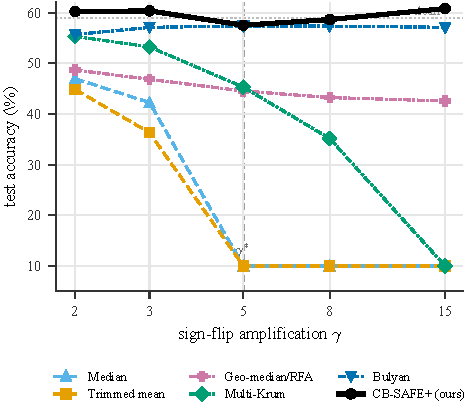
\includegraphics[width=\columnwidth]{fig_gamma_basin.pdf}
\caption{Sign-flip amplification sweep (CIFAR-10, $f{=}0.2$, 3 seeds): test accuracy
vs $\gamma$. Coordinate-wise rules collapse for all $\gamma\ge\gamma^{*}{=}5$; dashed
lines mark chance and the clean baseline.}
\label{fig:gamma-basin}
\end{figure}

\textbf{The full baseline panel confirms the mechanism} (Fig.~\ref{fig:dynamics},
Fig.~\ref{fig:acc-vs-f}, Table~\ref{tab:signflip}). Averaged over three seeds, the eight rules separate into
three regimes at $f{=}0.3$: the coordinate-wise rules (mean, trimmed mean, median)
are laundered to chance ($\approx$10\%) and the robust geometric median RFA
\cite{rfa} degrades to $\sim$20\%, confirming that location- and magnitude-based
aggregation fails regardless of sophistication; the vector-selection family degrades
but falls (Multi-Krum 21\%, Bulyan \cite{bulyan} 35\%); and only CB-SAFE+ holds near the
clean baseline at 57.4\%, whereas FedGT's actual BCJR decoder \cite{fedgt}, run per
round, degrades to 34\% on CIFAR-10 (and collapses to near-chance on FashionMNIST and
EMNIST) at this contamination by over-excluding honest clients
(Table~\ref{tab:detect}). That RFA collapses while Bulyan merely degrades sharpens
Proposition~\ref{prop:launder}: laundering specifically defeats rules that trust the
\emph{aggregate} direction or magnitude, precisely what cluster averaging preserves
for the attacker, whereas whole-vector selection resists longer.

\begin{table}[t]
\caption{Attacker identification, CIFAR-10 sign-flip ($N{=}30$, 3 seeds): attackers
caught ($\uparrow$) and honest false positives ($\downarrow$). FedGT is its real BCJR
decoder~\cite{fedgt}. Best in bold.}
\label{tab:detect}
\centering
\footnotesize
\setlength{\tabcolsep}{4pt}
\begin{tabular}{@{}lcccccc@{}}
\toprule
& \multicolumn{2}{c}{$f{=}0.1$} & \multicolumn{2}{c}{$f{=}0.2$} & \multicolumn{2}{c}{$f{=}0.3$}\\
\cmidrule(lr){2-3}\cmidrule(lr){4-5}\cmidrule(l){6-7}
Method & caught$\uparrow$ & FP$\downarrow$ & caught$\uparrow$ & FP$\downarrow$ & caught$\uparrow$ & FP$\downarrow$\\
\midrule
FedGT~\cite{fedgt}  & 2.7/3 & 13.0 & 5.3/6 & 17.7 & 7.7/9 & 11.0\\
CB-SAFE+ (ov1)   & 3/3 & 0.7 & 4/6 & 0.7 & 6.3/9 & 1.3\\
CB-SAFE+ hybrid  & \textbf{3/3} & \textbf{0.3} & \textbf{6/6} & \textbf{0.3} & \textbf{9/9} & \textbf{0.0}\\
\bottomrule
\end{tabular}
\end{table}

\textbf{CB-SAFE+ restores learning past the static breakdown}
(Table~\ref{tab:signflip}). With loss-probe
flags and temporal suspicion, the defense identifies all 3 of 3 attackers at
$f{=}0.1$ (60.5\%, at the clean ceiling) and all 9 sign-flip attackers
with \emph{zero} honest false positives at $f{=}0.3$ (three-seed means in Table~\ref{tab:detect}), recovering to 57.4\%
accuracy where every static coordinate-wise rule sat at 10\% and Multi-Krum at
21.4\%---exceeding even the 39--41\% the median achieves \emph{without any privacy}
($c{=}1$), i.e., the defense refunds the privacy dial's cost in rounds rather than
anonymity. At $f{=}0.2$ it holds 57.5\% while Multi-Krum reaches only 45.3\%, so the
defense's advantage over vector-selection rules grows with attack severity.
Under label flipping (a weak attack in this regime: all rules land within
44--52\%) the probe flags only the worst clusters and excludes conservatively (zero
false positives at $f{=}0.2$), matching the best static rule.

\textbf{Backdoor: a mechanism-independent blind spot.} The trigger attack leaves
main-task accuracy intact for every rule (50--55\%) while ASR stays at 86--97\%
across mean, trimmed mean, Multi-Krum, \emph{and} CB-SAFE+:
backdoored cluster sums \emph{reduce} clean root loss
and align with the honest direction, so they are invisible to loss- and
direction-based tests alike. Among the rules compared here, the partial exception at
$f{=}0.1$ is the coordinate-wise median, which suppresses ASR to 67\% on CIFAR-10
(and to 42\% on FashionMNIST): order statistics can filter the trigger direction's
coordinates when contamination is sparse. We therefore claim CB-SAFE+ for \emph{untargeted} model
poisoning only; targeted trigger attacks under secure aggregation remain open,
consistent with their difficulty even without privacy constraints, and we do not
position CB-SAFE+ against defenses built for them.


\subsection{Generalization Across Datasets and Modalities}\label{sec:general}
To test whether the laundering effect and CB-SAFE+'s recovery are artifacts of one
dataset, we repeat the sign-flip evaluation on three further benchmarks, each with
three seeds: FashionMNIST (a second image task on the same CNN), EMNIST-balanced (47
classes, a harder label space), and Edge-IIoTset (tabular IoT/IIoT intrusion
detection with a multilayer perceptron, a different modality in the security domain
of the closest prior work \cite{byzpqfl2026}). The pattern is identical everywhere
(Table~\ref{tab:signflip}, Fig.~\ref{fig:dynamics}): every coordinate-wise rule
collapses to chance at $f{\ge}0.2$ (10.0\% on the 10-class image sets, 7.3\% on
15-class Edge-IIoTset), Multi-Krum degrades gracefully then falls at $f{=}0.3$, and
CB-SAFE+ tracks the clean baseline. The round-by-round view
(Fig.~\ref{fig:dynamics}) shows this is not an endpoint artifact: the static rules
decay progressively while CB-SAFE+ dips during warmup and recovers as exclusions
fire. At $f{=}0.3$ CB-SAFE+ retains $\sim$95\%, $\sim$99\%,
and $\sim$99\% of the no-attack accuracy on CIFAR-10, FashionMNIST, and Edge-IIoTset
respectively, versus 12--18\% for the worst static rule. Pooling all 36 matched
(dataset, $f$, seed) cells, CB-SAFE+ beats \emph{every} baseline under a paired
$t$-test with Holm correction across the eight comparisons: the mean by 56.8 points
($p{<}10^{-15}$), trimmed mean by 45.5 and median by 43.5 (both $p{<}10^{-9}$),
geometric median by 20.9 ($p{<}10^{-4}$), Multi-Krum by 18.1 ($p{<}10^{-4}$), FedGT's
actual BCJR decoder by 18.3 ($p{<}10^{-4}$), Bulyan by 12.4 ($p{=}0.007$), and
FLTrust by 5.0 ($p{<}10^{-9}$).

Two qualifications on that test. It pools heterogeneous configurations, so it
establishes a population-level ordering, not a per-cell one: at individual cells the
ranking does change hands---FedGT ties CB-SAFE+ on FashionMNIST at $f{=}0.1$ and
leads it on Edge-IIoTset at $f{=}0.2$ (65.6 vs 65.2), and Bulyan leads at
Edge-IIoTset $f{=}0.1$. Per-cell values are in Table~\ref{tab:signflip} and should be
read directly. Second, the cells are not independent (three seeds share a dataset and
fraction), so the $p$-values are indicative rather than exact; the weakest comparison,
Bulyan, is the one to weigh, and it is also the rule operating furthest outside its
own precondition (Section~\ref{sec:baselines-config}). The
Edge-IIoTset result is the sharpest: at $f{=}0.3$ CB-SAFE+ holds 64.5\% against a
$\sim$65\% clean baseline while mean, trimmed mean, and median all sit at 7.4\%.
FLTrust is the one baseline that also withstands laundering on this dataset,
trailing CB-SAFE+ by 2.0 points there (62.5\% vs 64.5\%); that is the smallest
margin we report, which is why it is tested explicitly above.

\begin{table*}[t]\centering\footnotesize
\caption{Test accuracy (\%) under the sign-flip (laundering) attack across four datasets and malicious fractions $f$ (mean\,$\pm$\,std over 3 seeds for CIFAR-10/FashionMNIST; single seed for EMNIST/Edge-IIoTset). Higher is better; best per column in bold.}
\label{tab:signflip}
\setlength{\tabcolsep}{4pt}
\begin{tabular}{@{}lcccccccccccc@{}}\toprule
& \multicolumn{3}{c}{CIFAR-10} & \multicolumn{3}{c}{FashionMNIST} & \multicolumn{3}{c}{EMNIST} & \multicolumn{3}{c}{Edge-IIoTset}\\
\cmidrule(lr){2-4}\cmidrule(lr){5-7}\cmidrule(lr){8-10}\cmidrule(l){11-13}
Method & $f{=}.1$ & $f{=}.2$ & $f{=}.3$ & $f{=}.1$ & $f{=}.2$ & $f{=}.3$ & $f{=}.1$ & $f{=}.2$ & $f{=}.3$ & $f{=}.1$ & $f{=}.2$ & $f{=}.3$\\\midrule
FedAvg (mean) & 21.4\,{\scriptsize$\pm$8.3} & 10.0\,{\scriptsize$\pm$0.0} & 10.0\,{\scriptsize$\pm$0.0} & 48.9\,{\scriptsize$\pm$28.5} & 10.0\,{\scriptsize$\pm$0.0} & 10.0\,{\scriptsize$\pm$0.0} & -- & -- & -- & 27.0 & 7.3 & 7.3\\
Trimmed mean & 45.4\,{\scriptsize$\pm$2.4} & 10.0\,{\scriptsize$\pm$0.0} & 10.0\,{\scriptsize$\pm$0.0} & -- & -- & -- & -- & -- & -- & 58.0 & 11.7 & 7.3\\
Median & 47.8\,{\scriptsize$\pm$3.2} & 10.0\,{\scriptsize$\pm$0.0} & 10.0\,{\scriptsize$\pm$0.0} & 83.6\,{\scriptsize$\pm$1.1} & 10.0\,{\scriptsize$\pm$0.0} & 10.0\,{\scriptsize$\pm$0.0} & -- & -- & -- & 59.6 & 13.6 & 7.3\\
Multi-Krum & 53.6\,{\scriptsize$\pm$0.8} & 39.8\,{\scriptsize$\pm$2.2} & 20.3\,{\scriptsize$\pm$10.1} & \textbf{85.9\,{\scriptsize$\pm$0.8}} & 83.0\,{\scriptsize$\pm$1.6} & 43.1\,{\scriptsize$\pm$23.9} & -- & -- & -- & \textbf{63.3} & 59.4 & 38.5\\
CB-SAFE+ (ours) & 53.0\,{\scriptsize$\pm$0.6} & 47.1\,{\scriptsize$\pm$2.6} & 37.9\,{\scriptsize$\pm$12.6} & 85.7\,{\scriptsize$\pm$0.5} & \textbf{86.0\,{\scriptsize$\pm$0.5}} & \textbf{83.1\,{\scriptsize$\pm$1.9}} & -- & -- & -- & 61.9 & \textbf{62.3} & \textbf{61.5}\\
CB-SAFE+ hybrid (ours) & \textbf{53.9\,{\scriptsize$\pm$0.5}} & \textbf{49.5\,{\scriptsize$\pm$3.4}} & \textbf{50.0\,{\scriptsize$\pm$2.2}} & -- & -- & -- & -- & -- & -- & -- & -- & --\\
\bottomrule\end{tabular}\end{table*}


\begin{figure}[t]
\centering
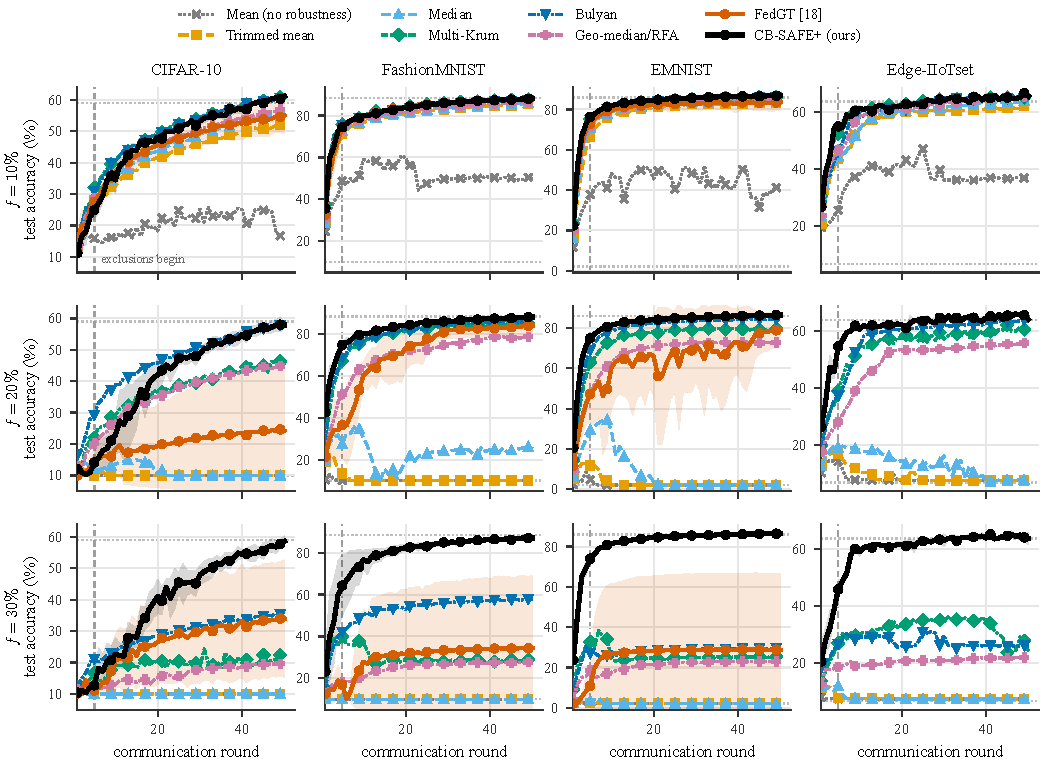
\includegraphics[width=\columnwidth]{fig_dynamics_signflip.pdf}
\caption{Training dynamics under sign-flip: test accuracy vs round, eight rules
across four datasets (columns) $\times$ malicious fraction $f$ (rows). Mean over 3
seeds; $\pm1$ SD bands for CB-SAFE+ and FedGT (real BCJR~\cite{fedgt}).
Dashed line: warmup $W{=}5$.}
\label{fig:dynamics}
\end{figure}

\begin{figure*}[tp]
\centering
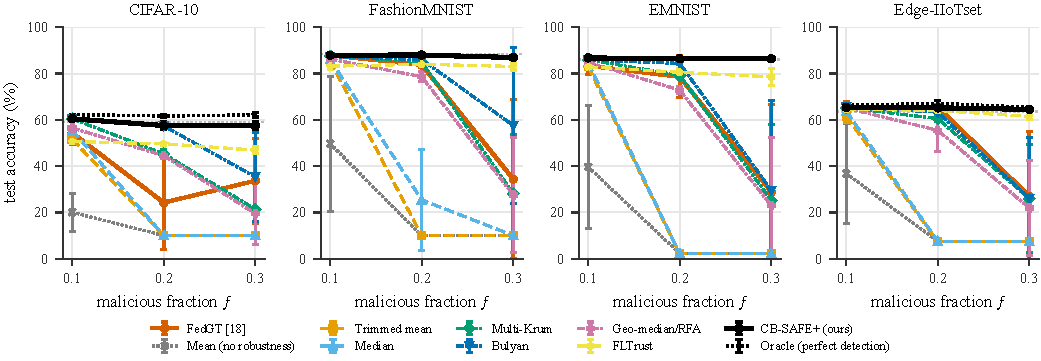
\includegraphics[width=\textwidth]{fig_acc_vs_f.pdf}
\caption{Final test accuracy vs.\ malicious fraction $f$ under sign-flip (mean over 3
seeds, 50 rounds; error bars $\pm$1 SD), one panel per dataset. The coordinate-wise
rules (mean, trimmed mean, median) and the geometric median collapse to chance by
$f{=}0.2$; Multi-Krum and Bulyan degrade then fall at $f{=}0.3$; only CB-SAFE+ tracks
the clean baseline (grey dotted) across all four datasets, staying within a few points
of the oracle (black dotted: perfect detection, all malicious clients excluded from
round~1). This is the endpoint summary of the round-by-round view in
Fig.~\ref{fig:dynamics}.}
\label{fig:acc-vs-f}
\end{figure*}

\begin{figure}[t]
\centering
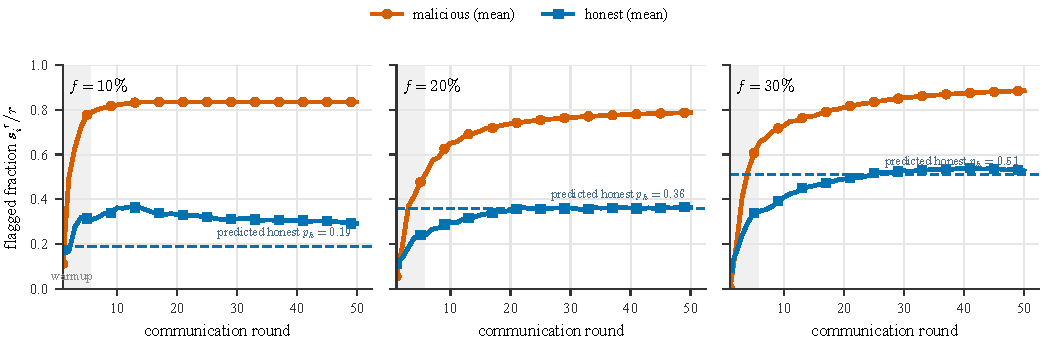
\includegraphics[width=\columnwidth]{fig_suspicion.pdf}
\caption{Temporal suspicion (CB-SAFE+, CIFAR-10): mean flagged fraction
$s_i^{\,r}/r$ for malicious vs honest clients, per fraction $f$ (3 seeds). Dashed:
predicted honest rate $p_h{=}1-(1-f)^{c-1}$; warmup shaded.}
\label{fig:suspicion}
\end{figure}

\subsection{Secondary Attack: Label Flipping}
Label flipping is a far milder attack than sign-flip, and it doubles as a control.
Table~\ref{tab:labelflip} shows that \emph{no} coordinate-wise rule collapses: the
undefended mean retains 53--64\% at $f{=}0.3$, versus 10\% under sign-flip. That
contrast isolates the laundering mechanism (Proposition~\ref{prop:launder}) as the
cause of the sign-flip failures, rather than any generic fragility of the setup.
CB-SAFE+ leads on the image benchmarks---on FashionMNIST it holds 87\% at
$f{=}0.3$ where the mean falls to 59\%---while on Edge-IIoTset all nine rules fall
within 4.0 points of one another, so the ordering there is a wash and trimmed mean
edges ahead at $f{=}0.2$ (66.3\% vs 64.3\%). We read that as the
control behaving as intended: with no laundering to exploit, robust aggregation has
little left to recover, so the separation that matters appears only under sign-flip. FedGT's actual BCJR decoder survives this
mild attack---unlike its sign-flip collapse---but trails CB-SAFE+ on CIFAR-10
($\sim$50--56\% vs $\sim$56--61\%) and is noisier between seeds, so even where its
accuracy signal is informative it is the less stable identifier.

\begin{table*}[t]\centering\footnotesize
\caption{Test accuracy (\%) under label-flip (four datasets $\times$ malicious fraction $f$; mean$\pm$std where shown, CIFAR-10/FashionMNIST baselines single-seed). FedGT is its real BCJR decoder~\cite{fedgt}; dash $=$ not evaluated. Best in bold.}
\label{tab:labelflip}
\setlength{\tabcolsep}{4pt}
\begin{tabular}{@{}lcccccccccccc@{}}\toprule
& \multicolumn{3}{c}{CIFAR-10} & \multicolumn{3}{c}{FashionMNIST} & \multicolumn{3}{c}{EMNIST} & \multicolumn{3}{c}{Edge-IIoTset}\\
\cmidrule(lr){2-4}\cmidrule(lr){5-7}\cmidrule(lr){8-10}\cmidrule(l){11-13}
Method & $f{=}.1$ & $f{=}.2$ & $f{=}.3$ & $f{=}.1$ & $f{=}.2$ & $f{=}.3$ & $f{=}.1$ & $f{=}.2$ & $f{=}.3$ & $f{=}.1$ & $f{=}.2$ & $f{=}.3$\\\midrule
FedAvg (mean) & \textbf{53.9} & 51.9 & 47.4 & 85.4 & 78.4 & 62.6 & 84.9 & 82.9 & 77.0 & \textbf{62.7} & \textbf{63.5} & 60.8\\
Trimmed mean & 52.7 & 51.1 & 47.3 & 85.6 & 78.7 & 77.0 & 85.4 & 83.5 & 80.0 & 62.5 & 62.7 & 60.5\\
Median & 52.0 & 51.2 & 44.8 & 85.5 & 84.7 & 75.2 & 85.6 & 83.6 & 78.2 & 61.5 & 62.7 & 59.7\\
Multi-Krum & 50.5 & 50.4 & 43.6 & 85.6 & 86.2 & 83.2 & 85.5 & 84.2 & 82.0 & 62.4 & 62.2 & 60.8\\
Bulyan & 50.9 & 49.0 & 43.7 & 85.2 & 85.5 & 81.9 & 85.2 & 84.2 & 81.5 & 61.2 & 61.6 & 60.5\\
Geo-median / RFA & 53.6 & 52.1 & 46.1 & 85.6 & 85.6 & 69.8 & 85.6 & 83.5 & 79.8 & 62.2 & 63.4 & 61.6\\
FLTrust & 25.7 & 26.3 & 25.0 & 75.4 & 75.3 & 73.0 & 50.0 & 48.2 & 44.8 & 37.4 & 38.2 & 37.1\\
FedGT~\cite{fedgt} & 48.1\,{\scriptsize$\pm$6.8} & 44.4\,{\scriptsize$\pm$6.4} & 47.6\,{\scriptsize$\pm$2.1} & 85.6\,{\scriptsize$\pm$0.5} & 85.0\,{\scriptsize$\pm$0.8} & 79.1\,{\scriptsize$\pm$5.7} & 84.7\,{\scriptsize$\pm$0.1} & 84.1\,{\scriptsize$\pm$1.4} & 81.2\,{\scriptsize$\pm$1.4} & $-$ & $-$ & $-$\\
\textbf{CB-SAFE+ (ours)} & 53.6 & \textbf{53.2} & \textbf{51.1} & \textbf{86.4} & \textbf{86.5} & \textbf{86.2} & \textbf{85.7\,{\scriptsize$\pm$0.2}} & \textbf{85.4\,{\scriptsize$\pm$0.2}} & \textbf{85.4\,{\scriptsize$\pm$0.1}} & 62.4 & 62.5 & \textbf{62.4}\\
\bottomrule\end{tabular}\end{table*}

\subsection{Adaptive Attackers}
\textbf{Amplitude-adaptive: choosing $\gamma$ to evade the loss probe.} The
direction flag fires on a loss margin $\delta$, so an attacker that knows the defense
should tune its amplitude $\gamma$ rather than maximize it: too large and every
cluster it touches is flagged, too small and the poisoning does little. We therefore
sweep $\gamma\in\{2,3,5,8,15\}$ at $f{=}0.2$ on CIFAR-10 (three seeds, 50 rounds) and
report, for each rule, the accuracy an attacker could force by picking its best
$\gamma$:

\begin{center}\footnotesize
\begin{tabular}{@{}lccccc@{}}\toprule
Rule & $\gamma{=}2$ & $\gamma{=}3$ & $\gamma{=}5$ & $\gamma{=}8$ & $\gamma{=}15$\\\midrule
Median & 47.0 & 42.3 & \textbf{10.0} & \textbf{10.0} & \textbf{10.0}\\
Multi-Krum & 55.3 & 53.2 & 45.3 & 35.2 & \textbf{10.0}\\
Bulyan & \textbf{55.7} & 57.1 & 57.4 & 57.3 & 57.1\\
CB-SAFE+ & 60.2 & 60.4 & \textbf{57.5} & 58.6 & 60.8\\
\bottomrule\end{tabular}
\end{center}

\noindent The worst case per rule is in bold. For the coordinate-wise median and
Multi-Krum an amplitude-adaptive attacker reaches chance ($10.0\%$); for CB-SAFE+ the
worst attainable value is $57.5\%$, at $\gamma{=}5$ --- the amplitude used throughout
the rest of this paper. The headline configuration is therefore already the
attacker's best choice against CB-SAFE+, and the basin is shallow: no $\gamma$ in the
sweep moves it more than $3.3$ points. Small $\gamma$ does not evade the probe,
because the suspicion score accumulates over rounds rather than requiring any single
round to exceed a margin. This is amplitude adaptivity only; a fully optimized
attacker in the style of \cite{fang2020,shejwalkar2021,baruch2019}, solving for the
update that maximizes damage subject to staying within the flag margin, is not
evaluated here and remains the strongest open threat to this design.

\textbf{Duty-cycled: poisoning intermittently.}
Suspicion-based exclusion invites an obvious evasion: poison only a fraction
$\delta$ of rounds, keeping most of the attack while holding the flagged fraction low
enough to blend into the honest side of the suspicion gap. We test this directly
(Table~\ref{tab:duty}), and it fails.
Because the partition is re-randomized every round, a resting attacker is still
flagged whenever it co-clusters with an \emph{active} one, so its accumulated
suspicion runs ahead of its nominal duty: even at a high duty $\delta{=}0.84$,
CB-SAFE+ still excludes all six attackers in every seed. Across
$\delta\in[0.5,1.0]$ accuracy never drops below $57\%$ (clean baseline $59\%$), where
coordinate-wise rules sit at $10\%$. At low duty the attacker evades most exclusions
($1.7$ of $6$ at $\delta{=}0.5$), but the attack is then too weak to matter
($59.8\%$, at the clean baseline); once $\delta{\geq}0.7$ the accumulated suspicion
catches essentially all six ($5.3$--$6.0$ of $6$). The
duty-cycler thus faces a no-win trade-off: raise $\delta$ and it is caught; lower it
and the attack is correspondingly weaker. A stronger
threshold-aware adversary that jointly minimizes footprint and detectability remains
open, but the naive duty-cycle evasion does not succeed.
\begin{table}[t]\centering\footnotesize
\caption{Adaptive duty-cycled attacker (CIFAR-10 sign-flip, $\gamma{=}5$, $f{=}0.2$,
$N{=}30$; mean\,$\pm$\,std over 3 seeds). A malicious client poisons a fraction
$\delta$ of rounds ($\delta{=}1$: always on); $\tau{=}0.85$ is the exclusion
threshold.}
\label{tab:duty}
\setlength{\tabcolsep}{6pt}
\begin{tabular}{@{}lcc@{}}\toprule
Attacker duty $\delta$ & Test acc.\ (\%) & Attackers excl.\ (of 6)\\\midrule
Clean (no attack) & $59.0$ & $-$\\
$0.50$ & $53.7$\,{\scriptsize$\pm$0.1} & $4.0$\\
$0.70$ & $52.5$\,{\scriptsize$\pm$1.0} & $6.0$\\
$0.80$ & $52.2$\,{\scriptsize$\pm$1.4} & $5.3$\\
$0.84$ & $51.3$\,{\scriptsize$\pm$2.2} & $6.0$\\
$0.90$ & $49.9$\,{\scriptsize$\pm$3.5} & $4.7$\\
$1.00$ (always-on) & $49.5$\,{\scriptsize$\pm$4.2} & $6.0$\\
\bottomrule\end{tabular}\end{table}


\subsection{Ablation: Which Component Earns the Robustness}
CB-SAFE+ layers three ingredients on top of clustered secure aggregation: temporal
reputation, temporally-overlapping re-randomized groups, and a windowed COMP decode.
Table~\ref{tab:ablation-variants} isolates each under the identical sign-flip
protocol. The base temporal reputation (ov1) restores learning at moderate
contamination and holds $53.6\%$ at $f{=}0.3$ on CIFAR-10; spreading the tests over
$o{=}4$ overlapping rounds (ov4) lifts this to $57.7\%$, and the full hybrid is
comparable at $57.4\%$, all far above FedGT's actual BCJR decoder, which collapses to
chance at this contamination (Table~\ref{tab:detect}). The decisive gain is the
temporal overlap; the windowed COMP decode, which counts a client only when it is
flagged across the whole window, mainly suppresses honest false positives rather than
adding accuracy. Both gains are concentrated on CIFAR-10, the hardest split: on FashionMNIST, EMNIST,
and Edge-IIoTset the three variants agree within $0.3$ points, where the base
temporal reputation already suffices, so the overlap and windowed decode earn their
keep specifically in the high-$f$, hard-task regime where laundering bites. The trust-free variant, which uses
\emph{no} root dataset, matches the others at $f{=}0.1$ but collapses beyond it:
attacker identification without any trusted anchor is possible only in the
low-contamination regime, a capability boundary of trust-free identification.

\begin{table*}[t]\centering\footnotesize
\caption{Ablation of CB-SAFE+ components under sign-flip (same protocol as Table~\ref{tab:signflip}). Overlapping groups and the hybrid COMP decode each add robustness at high $f$; the trust-free variant uses no root dataset but degrades beyond $f{=}0.1$. Best per column in bold.}
\label{tab:ablation-variants}
\setlength{\tabcolsep}{4pt}
\begin{tabular}{@{}lcccccccccccc@{}}\toprule
& \multicolumn{3}{c}{CIFAR-10} & \multicolumn{3}{c}{FashionMNIST} & \multicolumn{3}{c}{EMNIST} & \multicolumn{3}{c}{Edge-IIoTset}\\
\cmidrule(lr){2-4}\cmidrule(lr){5-7}\cmidrule(lr){8-10}\cmidrule(l){11-13}
Method & $f{=}.1$ & $f{=}.2$ & $f{=}.3$ & $f{=}.1$ & $f{=}.2$ & $f{=}.3$ & $f{=}.1$ & $f{=}.2$ & $f{=}.3$ & $f{=}.1$ & $f{=}.2$ & $f{=}.3$\\\midrule
Base: temporal reputation (ov1) & 61.1\,{\scriptsize$\pm$0.3} & 55.9\,{\scriptsize$\pm$1.8} & 53.6\,{\scriptsize$\pm$5.6} & \textbf{88.0\,{\scriptsize$\pm$0.4}} & \textbf{88.0\,{\scriptsize$\pm$0.3}} & 86.7\,{\scriptsize$\pm$1.0} & 86.7\,{\scriptsize$\pm$0.2} & 86.0\,{\scriptsize$\pm$0.2} & 86.3\,{\scriptsize$\pm$0.2} & 65.3\,{\scriptsize$\pm$0.4} & 65.1\,{\scriptsize$\pm$1.1} & \textbf{64.5\,{\scriptsize$\pm$0.7}}\\
\;+ overlapping groups (ov4) & 60.4\,{\scriptsize$\pm$0.6} & \textbf{57.6\,{\scriptsize$\pm$1.6}} & \textbf{57.7\,{\scriptsize$\pm$2.3}} & 87.9\,{\scriptsize$\pm$0.4} & 88.0\,{\scriptsize$\pm$0.3} & \textbf{86.9\,{\scriptsize$\pm$0.8}} & 86.7\,{\scriptsize$\pm$0.1} & 86.3\,{\scriptsize$\pm$0.1} & \textbf{86.5\,{\scriptsize$\pm$0.2}} & \textbf{65.4\,{\scriptsize$\pm$0.5}} & \textbf{65.2\,{\scriptsize$\pm$0.2}} & 64.5\,{\scriptsize$\pm$0.8}\\
\;+ hybrid COMP decode (full) & 60.5\,{\scriptsize$\pm$0.5} & 57.5\,{\scriptsize$\pm$1.6} & 57.4\,{\scriptsize$\pm$1.8} & 87.9\,{\scriptsize$\pm$0.3} & 88.0\,{\scriptsize$\pm$0.4} & 86.9\,{\scriptsize$\pm$0.8} & 86.7\,{\scriptsize$\pm$0.2} & \textbf{86.4\,{\scriptsize$\pm$0.1}} & 86.4\,{\scriptsize$\pm$0.2} & 65.4\,{\scriptsize$\pm$0.5} & 65.2\,{\scriptsize$\pm$0.2} & 64.5\,{\scriptsize$\pm$0.8}\\
Trust-free (no root data) & \textbf{61.4\,{\scriptsize$\pm$0.4}} & 10.0\,{\scriptsize$\pm$0.0} & 10.0\,{\scriptsize$\pm$0.0} & 87.8\,{\scriptsize$\pm$0.3} & 10.0\,{\scriptsize$\pm$0.0} & 10.0\,{\scriptsize$\pm$0.0} & \textbf{86.8\,{\scriptsize$\pm$0.1}} & 2.1\,{\scriptsize$\pm$0.0} & 2.1\,{\scriptsize$\pm$0.0} & 64.4\,{\scriptsize$\pm$0.3} & 45.2\,{\scriptsize$\pm$26.6} & 7.4\,{\scriptsize$\pm$0.2}\\
\bottomrule\end{tabular}\end{table*}

\subsection{The Privacy--Robustness Dial, Measured}

Fixing the rule (median) and sweeping cluster size traces the dial empirically
(CIFAR-10 sign-flip, a 30-round median-only sweep). Without privacy ($c{=}1$), the median degrades gently from
50\% to 39\% as $f$ grows to $0.3$, i.e., classical robust aggregation. At $c{=}3$ the
same rule holds to $f{=}0.1$ (48\%) and collapses beyond; at $c{=}5$ degradation
begins already at $f{=}0.1$ (40\%): the breakdown frontier shifts left exactly as
$(1-f)^c$ predicts. Two further observations sharpen the
picture. First, at $f{=}0.05$ privacy is \emph{free}: $c{=}3$ matches or
slightly exceeds $c{=}1$ (52\% vs.\ 50\%), because cluster averaging denoises
before the median. Second, the dial's cost is refundable: at $c{=}3$, $f{=}0.3$,
where the private median collapses to 10\% against $\sim$39\% without privacy,
CB-SAFE+ recovers comparable accuracy \emph{while keeping the anonymity set},
by paying in rounds (warmup) rather than in privacy. Overlapping groups add further
margin: the full detector at $o{=}4$ raises CIFAR $f{=}0.3$ from $53.6\%$ ($o{=}1$)
to $57.7\%$ (Table~\ref{tab:ablation-variants}).



\section{Security Discussion and Limitations}
\textbf{What the design guarantees.} Within a cluster, privacy reduces to the
double-masking argument of \cite{bonawitz2017} with the DH-style key agreement
replaced by an IND-CCA2 KEM: masks are ChaCha20 outputs keyed by HKDF of
encapsulated secrets, so an honest-but-curious server colluding with fewer than $t$
cluster members learns only cluster sums. The robust layer never inspects anything
finer than a cluster mean. \textbf{What it does not.} We do not claim security
against an actively malicious server (who could misreport dropouts; standard
mitigations apply), nor differential privacy on the cluster sums themselves; the
anonymity set is bounded by the alive cluster size, and cluster sums of very small
clusters leak more than full-cohort sums. Robustness degrades predictably as
$k(1-f)^c$ approaches the trim capacity: at $c{=}3$, $f{=}0.3$ leaves an expected
$3.4$ clean clusters of 10, near the breakdown of a 2-per-side trimmed mean; this
is the price of the anonymity set. HQC
operations are $\sim$100--600$\times$ slower than ML-KEM's depending on the operation, which is immaterial here
(setup-only) but would matter for protocols that encapsulate per round.

\section{Conclusion}
CB-SAFE positions cryptographic diversity as a configuration choice rather than a
research programme: the KEM sits behind one interface, and the measured cost of
choosing the code-based occupant is a one-time setup constant. The more consequential
finding is what secure aggregation does to robustness: cluster averaging does not
merely dilute poisoning, it \emph{launders} it, transforming conspicuous attacks
into plausible-looking sums that defeat exactly the rules practitioners would reach
for. Defending therefore requires signals that survive aggregation (direction,
loss) accumulated over time. CB-SAFE+ shows one such design that identifies
individual attackers from group observations without spending any privacy. The open
questions our results make concrete: targeted backdoors remain invisible to
sum-level probes at every malicious fraction we tested, an actively malicious server
is outside our threat model, and while a naive duty-cycled attacker does not evade
the temporal test (Table~\ref{tab:duty}), a threshold-aware adversary that jointly
minimizes its footprint and detectability remains the natural next step. The implementation and all measurement scripts are
released open-source as a reference point for KEM-level cryptographic diversity
in post-quantum secure aggregation for FL.

\begin{thebibliography}{9}
\bibitem{bonawitz2017} K.\ Bonawitz \emph{et al.}, ``Practical secure aggregation
for privacy-preserving machine learning,'' in \emph{Proc.\ ACM CCS}, 2017,
pp.\ 1175--1191.
\bibitem{nistir8545} National Institute of Standards and Technology, ``Status report
on the fourth round of the NIST post-quantum cryptography standardization process,''
NIST IR 8545, Mar.\ 2025.
\bibitem{fips203} National Institute of Standards and Technology,
``Module-lattice-based key-encapsulation mechanism standard,'' FIPS 203, Aug.\ 2024.
\bibitem{pqsf2024} X.\ Zhang, H.\ Deng, R.\ Wu, J.\ Ren, and Y.\ Ren, ``PQSF:
Post-quantum secure privacy-preserving federated learning,'' \emph{Sci.\ Rep.},
vol.\ 14, Art.\ no.\ 23553, 2024.
\bibitem{qinxu2025} X.\ Qin and R.\ Xu, ``Efficient post-quantum cross-silo
federated learning based on key homomorphic pseudo-random function,''
\emph{Mathematics}, vol.\ 13, no.\ 9, Art.\ no.\ 1404, 2025.
\bibitem{narsimhulu2026} P.\ Narsimhulu, P.\ Chithaluru, and R.\ Aluvalu,
``Efficient post-quantum cryptographic signature aggregation for low-latency
distributed networks,'' \emph{EURASIP J.\ Inf.\ Secur.}, vol.\ 2026, Art.\ no.\ 6, 2026.
\bibitem{byzpqfl2026} M.\ Rahmati and N.\ Rahmati, ``Byzantine-robust federated learning framework with
post-quantum secure aggregation for real-time threat intelligence sharing in
critical IoT infrastructure,'' arXiv:2601.01053, 2026.
\bibitem{cqsa2026} A.\ Nath and H.\ Kasyap, ``CQSA: Byzantine-robust clustered quantum secure aggregation in
federated learning,'' in \emph{Proc.\ Int.\ Workshop Secure Efficient Federated Learning (FL@ACM CCS)}, 2026.
\bibitem{lpnsecagg2026} ``Post-quantum secure aggregation via code-based homomorphic
encryption,'' arXiv:2601.13031, 2026.
\bibitem{comp} C.\ L.\ Chan, P.\ H.\ Che, S.\ Jaggi, and V.\ Saligrama,
``Non-adaptive probabilistic group testing with noisy measurements: Near-optimal
bounds with efficient algorithms,'' in \emph{Proc.\ 49th Annu.\ Allerton Conf.\
Commun., Control, Comput.}, 2011, pp.\ 1832--1839.
\bibitem{singh2025pqfog} J.\ Singh, P.\ Singh, A.\ Kaur, and M.\ Hedabou,
``Post-quantum secure fog-edge computing using federated learning with blockchain,''
\emph{J.\ Supercomput.}, vol.\ 81, Art.\ no.\ 1249, 2025.
\bibitem{fltrust} X.\ Cao, M.\ Fang, J.\ Liu, and N.\ Z.\ Gong, ``FLTrust:
Byzantine-robust federated learning via trust bootstrapping,'' in \emph{Proc.\ NDSS},
2021.
\bibitem{zeno} C.\ Xie, S.\ Koyejo, and I.\ Gupta, ``Zeno: Distributed stochastic
gradient descent with suspicion-based fault-tolerance,'' in \emph{Proc.\ ICML}, 2019.
\bibitem{bell2020} J.\ H.\ Bell, K.\ A.\ Bonawitz, A.\ Gasc\'on, T.\ Lepoint, and
M.\ Raykova, ``Secure single-server aggregation with (poly)logarithmic overhead,''
in \emph{Proc.\ ACM CCS}, 2020, pp.\ 1253--1269.
\bibitem{blanchard2017} P.\ Blanchard, E.\ M.\ El Mhamdi, R.\ Guerraoui, and
J.\ Stainer, ``Machine learning with adversaries: Byzantine tolerant gradient
descent,'' in \emph{Proc.\ NeurIPS}, 2017, pp.\ 119--129.
\bibitem{yin2018} D.\ Yin, Y.\ Chen, R.\ Kannan, and P.\ Bartlett,
``Byzantine-robust distributed learning: Towards optimal statistical rates,'' in
\emph{Proc.\ ICML}, 2018, pp.\ 5650--5659.
\bibitem{bagdasaryan2020} E.\ Bagdasaryan, A.\ Veit, Y.\ Hua, D.\ Estrin, and
V.\ Shmatikov, ``How to backdoor federated learning,'' in \emph{Proc.\ AISTATS},
2020, pp.\ 2938--2948.
\bibitem{brea2021} J.\ So, B.\ G\"uler, and A.\ S.\ Avestimehr,
``Byzantine-resilient secure federated learning,'' \emph{IEEE J.\ Sel.\ Areas
Commun.}, vol.\ 39, no.\ 7, pp.\ 2168--2181, 2021.
\bibitem{nguyen2025lattice} H.\ Nguyen, S.\ Huda, Y.\ Nogami, and T.\ T.\ Nguyen,
``Security in post-quantum era: A comprehensive survey on lattice-based
algorithms,'' \emph{IEEE Access}, vol.\ 13, pp.\ 89003--89024, 2025.
\bibitem{fedgt} M.\ Xhemrishi, J.\ \"Ostman, A.\ Wachter-Zeh, and A.\ Graell~i~Amat,
``FedGT: Identification of malicious clients in federated learning with secure
aggregation,'' \emph{IEEE Trans.\ Inf.\ Forensics Security}, vol.\ 20,
pp.\ 2577--2592, 2025.
\bibitem{bulyan} E.\ M.\ El Mhamdi, R.\ Guerraoui, and S.\ Rouault, ``The hidden
vulnerability of distributed learning in Byzantium,'' in \emph{Proc.\ ICML}, 2018,
pp.\ 3521--3530.
\bibitem{rfa} K.\ Pillutla, S.\ M.\ Kakade, and Z.\ Harchaoui, ``Robust aggregation
for federated learning,'' \emph{IEEE Trans.\ Signal Process.}, vol.\ 70,
pp.\ 1142--1154, 2022.
\bibitem{fang2020} M.\ Fang, X.\ Cao, J.\ Jia, and N.\ Z.\ Gong, ``Local model
poisoning attacks to Byzantine-robust federated learning,'' in \emph{Proc.\ USENIX
Security}, 2020, pp.\ 1605--1622.
\bibitem{shejwalkar2021} V.\ Shejwalkar and A.\ Houmansadr, ``Manipulating the
Byzantine: Optimizing model poisoning attacks and defenses for federated learning,''
in \emph{Proc.\ NDSS}, 2021.
\bibitem{flame2022} T.\ D.\ Nguyen \emph{et al.}, ``FLAME: Taming backdoors in
federated learning,'' in \emph{Proc.\ USENIX Security}, 2022, pp.\ 1415--1432.
\bibitem{mcmahan2017} B.\ McMahan, E.\ Moore, D.\ Ramage, S.\ Hampson, and
B.\ A.\ y~Arcas, ``Communication-efficient learning of deep networks from
decentralized data,'' in \emph{Proc.\ AISTATS}, 2017, pp.\ 1273--1282.
\bibitem{kairouz2021} P.\ Kairouz \emph{et al.}, ``Advances and open problems in
federated learning,'' \emph{Found.\ Trends Mach.\ Learn.}, vol.\ 14, no.\ 1--2,
pp.\ 1--210, 2021.
\bibitem{zhu2019} L.\ Zhu, Z.\ Liu, and S.\ Han, ``Deep leakage from gradients,''
in \emph{Proc.\ NeurIPS}, 2019, pp.\ 14747--14756.
\bibitem{geiping2020} J.\ Geiping, H.\ Bauermeister, H.\ Dr\"oge, and M.\ Moeller,
``Inverting gradients: How easy is it to break privacy in federated learning?,''
in \emph{Proc.\ NeurIPS}, 2020, pp.\ 16937--16947.
\bibitem{fredrikson2015} M.\ Fredrikson, S.\ Jha, and T.\ Ristenpart, ``Model
inversion attacks that exploit confidence information and basic countermeasures,''
in \emph{Proc.\ ACM CCS}, 2015, pp.\ 1322--1333.
\bibitem{shokri2017} R.\ Shokri, M.\ Stronati, C.\ Song, and V.\ Shmatikov,
``Membership inference attacks against machine learning models,'' in
\emph{Proc.\ IEEE Symp.\ Secur.\ Privacy}, 2017, pp.\ 3--18.
\bibitem{elkordy2022} A.\ R.\ Elkordy, J.\ Zhang, Y.\ H.\ Ezzeldin, K.\ Psounis,
and S.\ Avestimehr, ``How much privacy does federated learning with secure
aggregation guarantee?,'' \emph{Proc.\ Privacy Enhancing Technol.}, 2022,
pp.\ 510--526.
\bibitem{lightsecagg} J.\ So \emph{et al.}, ``LightSecAgg: A lightweight and
versatile design for secure aggregation in federated learning,'' in
\emph{Proc.\ MLSys}, 2022, pp.\ 694--720.
\bibitem{swiftagg} T.\ Jahani-Nezhad, M.\ A.\ Maddah-Ali, S.\ Li, and G.\ Caire,
``SwiftAgg: Communication-efficient and dropout-resistant secure aggregation for
federated learning with worst-case security guarantees,'' in \emph{Proc.\ IEEE
ISIT}, 2022, pp.\ 103--108.
\bibitem{shor1997} P.\ W.\ Shor, ``Polynomial-time algorithms for prime
factorization and discrete logarithms on a quantum computer,'' \emph{SIAM
J.\ Comput.}, vol.\ 26, no.\ 5, pp.\ 1484--1509, 1997.
\bibitem{mceliece1978} R.\ J.\ McEliece, ``A public-key cryptosystem based on
algebraic coding theory,'' \emph{JPL Deep Space Netw.\ Prog.\ Rep.}, pp.\ 114--116,
1978.
\bibitem{macwilliams1977} F.\ J.\ MacWilliams and N.\ J.\ A.\ Sloane, \emph{The
Theory of Error-Correcting Codes}.\ Amsterdam, The Netherlands: North-Holland,
1977.
\bibitem{fips204} National Institute of Standards and Technology,
``Module-lattice-based digital signature standard,'' FIPS 204, Aug.\ 2024.
\bibitem{baruch2019} G.\ Baruch, M.\ Baruch, and Y.\ Goldberg, ``A little is
enough: Circumventing defenses for distributed learning,'' in \emph{Proc.\ NeurIPS},
2019, pp.\ 8635--8645.
\bibitem{wangtails2020} H.\ Wang \emph{et al.}, ``Attack of the tails: Yes, you
really can backdoor federated learning,'' in \emph{Proc.\ NeurIPS}, 2020,
pp.\ 16070--16084.
\bibitem{tolpegin2020} V.\ Tolpegin, S.\ Truex, M.\ E.\ Gursoy, and L.\ Liu,
``Data poisoning attacks against federated learning systems,'' in \emph{Proc.\
ESORICS}, 2020, pp.\ 480--501.
\bibitem{fldetector2022} Z.\ Zhang, X.\ Cao, J.\ Jia, and N.\ Z.\ Gong,
``FLDetector: Defending federated learning against model poisoning attacks via
detecting malicious clients,'' in \emph{Proc.\ ACM KDD}, 2022, pp.\ 2545--2555.
\bibitem{dorfman1943} R.\ Dorfman, ``The detection of defective members of large
populations,'' \emph{Ann.\ Math.\ Stat.}, vol.\ 14, no.\ 4, pp.\ 436--440, 1943.
\bibitem{aldridge2019} M.\ Aldridge, O.\ Johnson, and J.\ Scarlett, ``Group
testing: An information theory perspective,'' \emph{Found.\ Trends Commun.\ Inf.\
Theory}, vol.\ 15, no.\ 3--4, pp.\ 196--392, 2019.
\bibitem{krizhevsky2009} A.\ Krizhevsky, ``Learning multiple layers of features
from tiny images,'' Univ.\ Toronto, Tech.\ Rep., 2009.
\bibitem{fashionmnist} H.\ Xiao, K.\ Rasul, and R.\ Vollgraf, ``Fashion-MNIST: A
novel image dataset for benchmarking machine learning algorithms,''
arXiv:1708.07747, 2017.
\bibitem{emnist} G.\ Cohen, S.\ Afshar, J.\ Tapson, and A.\ van~Schaik, ``EMNIST:
Extending MNIST to handwritten letters,'' in \emph{Proc.\ IJCNN}, 2017,
pp.\ 2921--2926.
\bibitem{edgeiiot} M.\ A.\ Ferrag, O.\ Friha, D.\ Hamouda, L.\ Maglaras, and
H.\ Janicke, ``Edge-IIoTset: A new comprehensive realistic cyber security dataset
of IoT and IIoT applications for centralized and federated learning,'' \emph{IEEE
Access}, vol.\ 10, pp.\ 40281--40306, 2022.
\bibitem{hsu2019} T.-M.\ H.\ Hsu, H.\ Qi, and M.\ Brown, ``Measuring the effects
of non-identical data distribution for federated visual classification,''
arXiv:1909.06335, 2019.
\bibitem{priroagg2024} S.\ Hou, S.\ Li, T.\ Jahani-Nezhad, and G.\ Caire, ``PriRoAgg:
Achieving robust model aggregation with minimum privacy leakage for federated
learning,'' \emph{IEEE Trans.\ Inf.\ Forensics Security}, 2024.
\bibitem{giskard2026} O.\ Touat, C.\ Sabater, M.\ Maouche, and S.\ Ben~Mokhtar,
``Giskard: Byzantine robust and confidential aggregation for large-scale decentralized
learning,'' arXiv:2606.19129, 2026.
\bibitem{flaegis2025} E.\ M\'armol~Campos, A.\ Gonz\'alez~Vidal, J.\ L.\
Hern\'andez~Ramos, and A.\ Skarmeta, ``FLAegis: A two-layer defense framework for
federated learning against poisoning attacks,'' arXiv:2508.18737, 2025.
\bibitem{safefl2025} Z.\ Dou, J.\ Wang, W.\ Sun, Z.\ Liu, and M.\ Fang, ``Toward
malicious clients detection in federated learning,'' arXiv:2505.09110, 2025.
\bibitem{flltd2026} D.\ K.\ Bhaskar, B.\ Minimol, and V.\ P.\ Binu, ``Robust federated
learning for malicious clients using loss trend deviation detection,''
arXiv:2601.20915, 2026.
\bibitem{flamingo} Y.\ Ma, J.\ Woods, S.\ Angel, A.\ Polychroniadou, and T.\ Rabin,
``Flamingo: Multi-round single-server secure aggregation with applications to private
federated learning,'' in \emph{Proc.\ IEEE Symp.\ Security and Privacy (S\&P)}, 2023,
pp.\ 477--496.
\bibitem{rofl} H.\ Lycklama, L.\ Burkhalter, A.\ Viand, N.\ K\"uchler, and A.\ Hithnawi,
``RoFL: Robustness of secure federated learning,'' in \emph{Proc.\ IEEE Symp.\ Security
and Privacy (S\&P)}, 2023, pp.\ 453--476.
\bibitem{eiffel} A.\ Roy~Chowdhury, C.\ Guo, S.\ Jha, and L.\ van~der~Maaten,
``EIFFeL: Ensuring integrity for federated learning,'' in \emph{Proc.\ ACM CCS}, 2022,
pp.\ 2535--2549.
\bibitem{elsa} M.\ Rathee, C.\ Shen, S.\ Wagh, and R.\ A.\ Popa, ``ELSA: Secure
aggregation for federated learning with malicious actors,'' in \emph{Proc.\ IEEE Symp.\
Security and Privacy (S\&P)}, 2023, pp.\ 1961--1979.
\bibitem{hqc} C.\ Aguilar~Melchor, N.\ Aragon, S.\ Bettaieb, L.\ Bidoux, O.\ Blazy,
J.-C.\ Deneuville, P.\ Gaborit, E.\ Persichetti, and G.\ Z\'emor, ``HQC: Hamming
Quasi-Cyclic,'' NIST Post-Quantum Cryptography Standardization, Round-4 submission,
2023.
\bibitem{shamir1979} A.\ Shamir, ``How to share a secret,'' \emph{Commun.\ ACM},
vol.\ 22, no.\ 11, pp.\ 612--613, 1979.
\bibitem{chacha20} D.\ J.\ Bernstein, ``ChaCha, a variant of Salsa20,'' in
\emph{Workshop Record of SASC}, 2008.
\bibitem{hkdf} H.\ Krawczyk, ``Cryptographic extraction and key derivation: The HKDF
scheme,'' in \emph{Proc.\ CRYPTO}, 2010, pp.\ 631--648.
\bibitem{bcjr} L.\ R.\ Bahl, J.\ Cocke, F.\ Jelinek, and J.\ Raviv, ``Optimal decoding
of linear codes for minimizing symbol error rate,'' \emph{IEEE Trans.\ Inf.\ Theory},
vol.\ 20, no.\ 2, pp.\ 284--287, 1974.
\end{thebibliography}

\end{document}
